\documentclass{article}
\usepackage{enumitem}
\usepackage{fixltx2e}
\usepackage{hyperref}
\usepackage{graphicx}
\usepackage{listings}
\usepackage{color}
\usepackage[tbtags]{amsmath}
\usepackage{textcomp}
\usepackage{subcaption}
\usepackage{longtable}
\usepackage{float}
\usepackage[top=25truemm,bottom=30truemm,left=25truemm,right=25truemm]{geometry}



\setlength\intextsep{5pt}
\setlength\textfloatsep{5pt}


\def\vector#1{\mbox{\boldmath $#1$}}
\begin{document}

\title{Structure of complex networks across domains}
\author{Kansuke Ikehara}
\maketitle

\begin{abstract}
The structure of complex networks has been of interest in many scientific and engineering disciplines over decades. A number of scientists have reported findings that indicated the characteristics of network structure that are claimed to be universal, such as \textit{small-worldness} and long tail degree distribution. Domain specific characteristics, for example specific profiles of network motifs and high-triangle density in social networks, have also been reported previously. However, there is no comprehensive study of inter-domain relationships of complex networks based on the network structure. In this paper, we study over 1000 of real-world networks of diverse domains ranging from ecological food-web to online social network along with networks generated from four popular network models. Our study is data-driven, utilizing machine learning techniques such as random forest and confusion matrix and we show the relationships among network domains in terms of network structure. Our result indicates that there are some pairs of network domains (categories) that are inherently hard to distinguish based purely on network structure. We have found that these domains tend to have similar underlying mechanisms which generate a network or drive the growth of a network or processes which take place on a network itself.
  
\end{abstract}
\tableofcontents

%%%%%%%%%%%%%%%% --- New Chapter --- %%%%%%%%%%%%%%%%
\newpage
\section{Introduction}
	\subsection{Complex Networks}
	Almost every scientific and engineering discipline deals with data that come from some sorts of experimental observations. Traditionally, such data are expressed as numbers, which may represent temperature, velocity, or voltage, and methodologies that analyze these numbers have been established for over hundreds of years. \textit{Graph} or \textit{network}, which is a kind of data representation describing the relations among some entities such as persons, molecules, animals, logical gates, etc., has been used as a new way to approach, interpret and solve real-world problems in the last decades. Social science, for instance, has witnessed the power of network analysis with the recent emergence of online social network services such as Facebook, Twitter, LinkedIn, etc. \cite{Kleinberg:1}. With the abundance of online data, faster and more efficient computational resources along with advancements of graph algorithms, previously invisible social phenomena at the scale of off-line social networks, which usually consist of tens to hundreds of nodes at most, have been observed in a large scale online social networks.  Biological sciences use networks as a tool to dissect biological, chemical and ecological processes in order to gain insight into the functionality of a brain that consists of networks of neurons \cite{BrainNetwork}, complex metabolic reactions within a human's cells and relationships between malfunctioning metabolic processes and human diseases \cite{MetabolicNetworkAndDiseases} and the effect in biodiversity, that might result from perturbation in an ecological network, such as food-web, mutualistic network, etc. \cite{EcologicalNetwork}. Engineering systems such as the Internet \cite{Internet}, power grids \cite{PowerGrid}, water distribution networks \cite{WaterDistribution}, transportation networks \cite{Train}, etc. have also been investigated with using network analysis tools for constructing more efficient and robust systems. 
	
	A term \textit{complex network} depicts an essential difference from ordinary graphs having some kinds of regular structure that have been studied in the field of mathematics for a long time: the structure of real world networks almost always exhibits an unusual pattern that greatly deviates from the regular structure and this seemingly irregular and complex structure can often be a clue to the underlying mechanism and/or phenomenon of the process of interest.  For example, the unusual density of triangles in social networks implies an underlying mechanism in our society: the formation of our social circles tends to be made by local interactions, such as introducing your friend to another friend in your circle that results in a new connection between your friends, making a triangle in the circle. There have been a number of studies that investigate the structure of complex networks of diverse fields and connections between the structure and the underlying mechanism of the process. In the next section we discuss them in the greater detail.
	
	\subsection{Common Properties in The Structure of Networks}
	The structure of a network can be characterized in a number of ways, but there are three structural properties that are found in nearly all types of networks: skewed degree distribution, small-worldness and community structure.
	
	 The degree of a node is a measure of how many edges are connected to a particular node, and the probability distribution $p(k)$ over all nodes essentially describes the "unfairness" in the network. If all of the nodes in a network have the exact same number of connections, the fairest case, then $p(k)$ behaves like Kronecker delta, where $p(k)$ has a value $1$ only at a specific degree $k$. Or if it is less fair, one may observe a narrow Gaussian-like distribution around an average degree. In the real world network, however, this almost never happens. What is observed most of the time instead, is a very skewed degree distribution in which most of the nodes have a few connections incident upon them, and very few nodes have a disproportionally large number of connections with them. \textit{Power-law} distribution is one of candidate distributions that describes the observed phenomenon well, and a network having this distribution is often called \textit{scale-free} network \cite{Barabasi99emergenceScaling}. Surprisingly, a number of networks  from diverse fields, such the Internet, metabolic reactions, World-Wide-Web, etc. have been claimed to be a scale-free network. However, one needs to be careful in order to validate if a network of interest indeed has the power-law degree distribution and there seems to be that a number of such claims need more statistically valid treatment such one proposed by Clauset \textit{et al.} for justification \cite{Clauset:PowerLaw}. The disproportionality of the skewed degree distribution indicates an existence of  \textit{hubs}, \textit{cores} or \textit{elites} in a network. Such important nodes in a network can play a critical role for a network to function properly and the failure of such nodes may result in a catastrophe \cite{ScaleFreeAttack}.
	
	The next common structural characteristic of networks is \textit{small-worldness}, first conceptually introduced by a Milgram's experiment \cite{Milgram} and mathematically proposed in a paper by Watts and Strogatz \cite{watts1998cds}. They proposed a random network model that, depending on the parameter setting, produces a network having properties as follows: 1. high density of triangles (clustering coefficient), implying that if three nodes are connected, it is likely that those three nodes actually compose a triangle; 2. low average distance between a pair of nodes, which indicates that from any node it is just a few steps, in average, to reach any other node in the network. These properties are accomplished by an existence of "long-range" connections bridging together pairs of nodes topologically far away from each other. Small-worldness holds seemingly contradicting properties together: the large degree of local-ness exhibited as a large clustering coefficient value and the large degree of global-ness expressed as a small value of mean geodesic distance.  These properties make small-world networks a very efficient system for information flow \cite{SmallWorldEfficiency} and synchronizing coupled oscillators in the network \cite{SmallWorldSynchronization}. Note that the small-worldness itself is orthogonal to the skewed degree distribution, meaning that so-called small-world networks can be constructed without the heavy-tail degree distribution. The definition of small world network presented above is, however, not generally used. Most of the researchers today refer small-world property to as simply the low average pairwise distance between nodes that grows approximately as $O(\log(n))$.
	
	
	Many of the real-world networks contain \textit{modules} or \textit{communities} in which nodes are densely connected but among which there are sparse edges running. This structure is called \textit{community structure} of a network and there has been a number of studies investigating such communities and inventing a new algorithm for detecting communities in the network \cite{Modularity1, Modularity2, ModularityReview}. The communities in a network found by algorithms often correspond to the functional units of the network: a unit of chemical reactions producing vital chemical product in the metabolic network, a group of densely connected neurons taking charge of a cognitive function, such as language and visual processing, and a group of scientists working together in the same field.
	
	
	
	\subsection{Distinguishing Structural Features of Networks}
The properties such as skewed-degree distribution, small-worldness and community structure are found in networks of various kinds, but they alone cannot explain a diversity of networks in terms of network structure. It has been believed by a number of researchers that some classes of network have a set of distinguishing structural features that makes the specific network class "stand out" among others. In this section we show some examples of network class that have distinguishing structural features, including social networks, brain networks and subway networks.

Social networks, regardless of whether they are off-line as we see in our daily lives or online like Facebook, have long been known for having  distinguishing structural features: clustering and positive degree assortativity \cite{AssortativeMixing,WhySocialNetworks, Mislove:2007:OnlineSocial}. The large degree of clustering indicates the high probability of one's friends being friends to each other and the positive degree assortativity shows a tendency that high-degree nodes (nodes having many connections) connect to other high-degree nodes while low-degree nodes connect to other low-degree nodes. Real-world networks, \textit{except} social networks, in general exhibit low clustering and negative degree assortativity that are almost in accordance with ones of their randomized counterparts or null models having the same degree distribution. As Newman pointed out in his paper \cite{WhySocialNetworks}, negative degree assortativity is a natural state for networks. Therefore, in order for a network to have positive degree assortativity, it needs a specific structure that favors the assortativity. The community structure of social networks, as mentioned in the paper, is the key aspect as to why they exhibit the properties, namely clustering and positive degree assortativity. People or nodes in social networks usually belong to some sort of groups or communities and people in the same community are likely to know each other. This community membership yields the high clustering in the social network.  For positive degree assortativity, the size of the communities may play an essential role: individuals in a small group can only have low degree whereas individuals in a large group can, potentially, have much larger degree. This approximate correspondence of degree in the groups is essentially degree assortativity itself.


Brain networks, often referred to as \textit{connectome}, have been in the focus of neuroscience in the last decade in order to solve the long-standing scientific question: \textit{How does a brain work?}  The field that studies extensively brain networks using a tool set from mathematics, computer science, etc., is called \textit{connectomics} and one of the recent research topics in this field is investigating how a topology of a brain network affects the brain's function \cite{ComparativeConnectome}. A number of studies show the topological feature of brain networks, including not only human brain but also other animals, is that: 1. they are highly modularly structured; 2. they have topological connections that are anatomically long, implying high cost of wiring, and make a brain network topologically small, like a small-world network; and 3. they have a core of highly connected nodes, called \textit{rich-club} in some literatures, that connect modules across the network together. The modular structure in a brain network is found to be correlating with a discrete physiological and cognitive function of a brain. The existence of topologically short yet anatomically long connections enables a brain to have an efficient way to process the information flowing on the network. The rich club of a brain network plays an important role of integrating information that is produced and processed in different parts of the brain and this integration of information enables animals including human beings to do complex tasks.

Networks of subways in the major cities around the world have an interesting common feature unique to them, that is \textit{core-branch} structure \cite{Train}. They have a ring-shape connections of stations and dense connections therein, referred to as the "core" of the network. In the core, stations are relatively densely connected to each other, enabling residents of a city to move around quickly. From the ring of the core, branches radiate outward connecting stations far from the center of the city. This structural feature is the result of balance between an efficiency of flow of people in a metro area and cost for constructing rail lines between stations \cite{SpatioalNetwork1,SpatioalNetwork2}. 


	
	\subsection{Comparison and Classification of Networks}
	 In the last decades, researchers from the wide range of fields including biology, social science and physics, have been interested in if there is any structural difference between different classes of networks, if there is a set of structural features unique to a specific network class and if there is any "family" of networks in which networks of different classes share the same structural patterns. These questions are usually converted into a problem of comparing and classifying networks according to some criteria and these criteria span from a simple feature such as clustering coefficient, to more complicated ones such as network motifs, which is going to be explained later.
	
	One of the earliest works in network comparison and classification was done by Faust and Skvoretz \cite{Faust.Skvoretz2002Comparing}, in which they compared various kinds of offline social networks, such as grooming relationships among monkeys, co-sponsorship among U.S. Senate of 1973-1974 and so on. Their comparison of networks is based on a statistical model that incorporates parameters each describing a characteristic network structural feature, for example the frequency of a cyclic triangle (here the networks are \textit{directed}, meaning that edges have directionality). The statistical model essentially predicts an existence of an edge $(i,j)$ in a network based on the parameters and the authors used such a statistical model "trained" on a network for predicting an edge in a different network. Their assumption is that if two networks are similar, a model trained on one of the pair should predict well an edge existence in another network. With this assumption they define the Euclidian distance as a function of a summation over all edge predictions, construct a distance matrix and project it onto a two dimensional space using a technique called Correspondence Analysis, which is similar to Principal Component Analysis. They have found the key insight that what makes networks similar in terms of structure is the property of of edges, namely a kind of relation. For example, networks describing agonistic relations, regardless of kinds of species, exhibit the similar network structure. Although this study was pioneering in graph comparison and classification, it only focused on offline social networks, which themselves are a very narrow field of study.
	
	The breakthrough in graph comparison and classification came along a series of papers by Milo \textit{et al.} that introduced the idea of \textit{network motifs} and "super family" of networks \cite{Milo_motif, Milo_SuperFamily}. Network motifs are essentially patterns of frequent sub-graph (motif) in a particular network compared to its randomized network\cite{Milo_motif}. They have shown each category of network, such as gene regulation (transcription), food webs, electronic circuits, etc., has a distinct pattern of network motifs. Essentially the distinction of patterns indicates the functional difference in those networks. Furthermore, they revealed the existence of super families of networks that are groups of network categories having the highly convergent motif profiles. These studies are, as far as we know, the first which investigated a diverse set of networks from different domains and found the underlying similarities among the network categories.
	
	One of the most recent studies in graph comparison and classification investigated 746 networks and constructed a taxonomy of such networks \cite{Onnela_Taxonomy}.  Onnela \textit{et al.} used a technique called \textit{mesoscopic response functions} (MRFS) that essentially describes the change of a specific value related to the community structure of a network with respect to a parameter $\xi \in [0,1]$. Each network has its own MRFS and they calculated the distance between networks which is defined as an area of difference between two networks' MRFS. Their framework successfully identifies groups of networks that are similar in terms of community structure.

	
	
	\subsection{Structural Diversity of Networks}
	A number of graph comparison and classification studies have only focused on finding features that make network categories distinguishable from other kinds and/or finding the groups or super families of networks that are structurally similar. With the abundance of available network data of various kinds and scales and the techniques from the field of machine learning, we could tackle the fundamental, yet unexplored question: \textit{What makes complex networks structurally diverse?} There has been a number of studies that try to discover or formulate an idea that explains the structural \textit{universality} of networks, including skewed degree distribution, small-world networks, community structure and so on. There is, however, no general theory that explains the structural \textit{diversity} of complex networks across a number of domains/fields. The aim of  this thesis is to establish such a general theory explaining the structural diversity of complex networks. Below are the three  questions we have formulated as research objectives:

\begin{enumerate}
	\item \textit{What aspects of network structure do make a specific category of network different from others?}
	\item \textit{Are there any sets of network categories that are inherently indistinguishable from each other based on network structure?} 
	\item \textit{If two networks of different categories are indistinguishable by network structure, are their mechanisms of underlying processes the same? And vice versa.}
\end{enumerate}

The first question is to, in some extent, an extension to the studies investigating social networks' structural strangeness. For example, what kinds of network structure are distinguishing, say metabolic networks from the other kinds? As far as we know, few previous studies have done extensive investigation in finding distinctive characteristics of specific kinds of networks compared to other kinds except social networks.

The second question asks if there is any structural similarity between different kinds of networks. We, however, use the word "indistinguishable" in stead of "similar" since we try to observe the commonality from a confusion matrix of a classifier, where a misclassified instance is considered to be indistinguishable from a class it was classified as because it is so similar to other instances of the wrong class, the algorithm fails to label the instance correctly.


The last question is essentially all about elucidating the meta-structure in the network domains. What if two very distinct categories (domain) of networks, say biological and technological ones, exhibit very similar network structure and a classifier misclassifies them many times? Is this because their underlying network generative processes, or their processes on networks themselves are the same? Answering this question helps us understand a mechanism for the formation of a specific network structure.


The contribution of answering those questions comes in two ways: first it gives us a general conceptual framework upon which networks are studied across domains. Previous studies have only looked at a single category or multiple categories as one category, ignoring the relationships between categories. By studying networks across domains, one could find general theories of networks or test a hypothesis across domains in a more plausible way.  For instance, one could test validity of a network model across all of domains and find out which domains the network model can explain well; second it gives us the knowledge base upon which various network-related algorithms could be constructed and tuned properly.  Many practical graph algorithms take no assumption in domain-specific network structure. It may be possible, however, to construct a new algorithm which runs faster and more efficiently on a specific kind of networks by taking into account of such domain-specific knowledge. For example, if there exists any unique network structural property of recommendation networks,  it may be applied to construct or fine tune a recommendation engine that utilizes knowledge of unique network structure. As the size of some real-world networks has grown to an unprecedented scale, domain-specific knowledge in network structure will be a key to analyze such large networks in a faster and more efficient way.

\subsection{Project Description}

In this thesis, we study approximately 1000 of various kinds of real-world networks, ranging from ecological food-web to online social network to digital circuit along with 580 of synthetic networks generated from four different models. We extract network statistics as features of a network, construct a high-dimensional feature space, where each axis corresponds to one of the network features, and map each network onto the feature space. We then train a machine learning algorithm called \textit{random forest} with the training set of network data in order to learn the function that relates structural features of networks to class labels, namely network domains and sub-domains. As the category distribution is skewed, meaning that some categories of networks have larger number of instances than the other minority categories, we try several sampling methods and show the effect of each methodology. We construct confusion matrices based upon classification results and proceed to analyze the misclassification with which we can answer research questions explained in the previous section. We then conclude with discussion based on several hypotheses and classification results.

%%%%%%%%%%%%%%%% --- New Chapter --- %%%%%%%%%%%%%%%%
\newpage
\section{What Is A Network?}
	\subsection{Formal Definition}
	Formally, a network or graph is a mathematical object consisting of a set of edges (arcs) and nodes (vertices), which can be written as $G = (E,V)$. In many cases, an \textit{adjacency matrix} is used as a representation of a network, where each element of the matrix $A_{ij}$ takes a binary value, $1$ for presence of an edge between nodes $i$ and $j$, and $0$ if there is no edge between these nodes in an unweighted network.  If edges of the network are weighted, meaning that  edges can have real values, then the network is called \textit{weighted}. Related with weighted networks is \textit{multigraph} in which any pair of nodes is allowed to have multiple edges connecting them. One should be careful here with the representation with an adjacency matrix for weighted network and multigraph, as the interpretation of the value of $A_{ij}$ depends on the context in which one treats the graph for the problem. For example, $A_{ij} = 2$ may describe an edge between $i$ and $j$ weighted by $2$, or there are \textit{two} edges running between $i$ and $j$. If the matrix is symmetric, namely $A_{ij} = A_{ji},  \forall i,j \in V$, the matrix represents an \textit{undirected} network in which edges do not have directionality at all. If the matrix is asymmetric, on the other hand, it's representing a \textit{directed} network, where edges have directionality. If the diagonal elements of a matrix $A$ are non-zero, the network has \textit{self-loops} which indicates that there are edges originating from and pointing to the exact same node. In many studies such self-loops are simply ignored for the sake of simplicity. The last, but not the least kind of network is \textit{bipartite network}, in which there are two groups of nodes and edges exist \textit{only} between nodes of different groups. An example of bipartite network is a network of cooperate board membership where there are groups of companies and board members and edges connect companies and board members. Often times, a bipartite network is converted into a network in which there is only one kind of nodes, for instance only board members in the case of cooperate board membership network, by an operation called one-mode projection. In the one-mode projected network of board members, an edge between persons $i$ and $j$ now represents the frequency that they sit on the same board for companies.
	
	As such, there are many kinds of networks, each describing networks differently. In our study, for the sake of simplicity and comparability, we focus on using a \textit{simple graph}, in which edges have no directionality and weight and there is no self-loops.
	
	\subsection{Structural Features of A Network}
	There are many ways to characterize a network in a quantitative manner that use the network's structural features \cite{Newman:NetworksIntro,NetworkCharacterizationSurvey}. Some network features, however, are implicitly correlated with the size of networks, which itself is a very strong feature: the number of nodes in web graphs is usually a magnitude of $10^6$ or more whereas ecological food webs contain usually less than 100 nodes. Examples of such features include, for instance, distance-related features such as average path length and network diameter that are believed to grow approximately in the order of $\log(n)$, where $n$ is the number of nodes in a network. Another structural feature correlated with the size of the network is the modularity of network \cite{Modularity1}. Simply put, modularity quantifies the degree to which how much an observed network can be "partitioned" into modules within which edges are densely present but between which edges are sparsely present. The derivation of modularity is essentially based on comparing the original network with a random network having the same degree distribution which is called configuration model and the value of modularity is practically the degree of difference between the original graph and its randomized counterpart. If the size of a network is large, the random network becomes so different that the modularity value becomes large as well \cite{ResolutionLimit}.
	
	The feature set we use in this study is scale-invariant, meaning that the size of network is supposed not to affect the value of a feature. This set of features allows us to compare networks without the notion of network size. In the following sections we describe important structural features that are relevant in this study.	
	 
	\subsubsection{Degree}
	The \textit{degree} of a node in a network is the number of edges attached to the node. For a node $i$ in an unweighted network, the degree $k_i$ of the node can be written mathematically as:
	
	\begin{equation}
 	 k_i = \sum_{j = 1}^n A_{ij}.
	\end{equation}

	
	\subsubsection{Clustering Coefficient}
	Clustering coefficient, which describes a degree of \textit{transitivity} in a network, is one of the most widely used metrics in network analysis especially in the context of social network. Transitivity in the context of networks means that if nodes $a$ and $b$ are connected as well as nodes $b$ and $c$, then nodes $a$ and $c$ are connected. Mathematically, the definition of clustering coefficient is given by the following equation:
	\begin{equation}
	C = \frac{\text{number of closed paths of length two}}{\text{number of paths of length two}}.
	\end{equation}
	
	\subsubsection{Degree Assortativity}
	\textit{Assortativity} in a network indicates a tendency for nodes to be connected to other nodes with similar node attribute. In a social network, for instance, node attributes which could be the basis for assortativity include language, age, income, alma mater, etc. On the other hand, \textit{disassortativity} exhibits nodes' tendency to be connected to other nodes having different node attribute in the network. An example network of disassortatvity would be a social network of heterosexual-relationship among people. 
	\textit{Degree assortativity} is a form of assortativity in which nodes with similar degree value tend to be connected together. Therefore in a network exhibiting high degree assortativity, there is a core of highly connected nodes with the high degree and periphery of nodes sparsely connected to other low-degree nodes.
	
	Here, we first derive a general \textit{assortativity coefficient} of an undirected, unweighted network based on scalar node attribute, excluding enumerative ones such as language, alma mater, etc., then we easily find \textit{degree assortativity coefficient}.
	
	First we calculate the covariance of $x_i$ and $x_j$ for the vertices at the ends of all edges, where $x_i$,$x_j$ are nodes $i$ and $j$'s attributes.
	The mean $\mu$ of the value of $x_i$ at the end of one edge is defined as:
	\begin{equation}
	\mu = \frac{ \sum_{ij}A_{ij}x_i }{\sum_{ij}A_{ij}} = \frac{\sum_i k_i x_i}{\sum_i k_i} = \frac{1}{2m}\sum_i k_i x_i,
	\end{equation}
where $k_i$ is a degree of node $i$.

Then, the covariance of of $x_i$ and $x_j$ over all edges is derived as:
	\begin{equation}
	\begin{split}
	\text{cov}(x_i, x_j)  &= \frac
					{ \sum_{ij}A_{ij}(x_i - \mu)(x_j - \mu) }
					{\sum_{ij}A_{ij} } \\
					&= \frac{1}{2m}\sum_{ij}A_{ij} (x_i x_j - \mu x_i - \mu x_j +\mu^2) \\
					&= \frac{1}{2m}\sum_{ij}A_{ij}x_i x_j - \mu^2 \\
					&= \frac{1}{2m}\sum_{ij}A_{ij}x_i x_j - \frac{1}{(2m)^2}\sum_{ij}k_i k_j x_i x_j \\
					&= \frac{1}{2m}\sum_{ij}(A_{ij} - \frac{k_i k_j}{2m})x_i x_j.
	\end{split}
	\end{equation}
This covariance will be positive if both $x_i$ and $x_j$ have, in average, similar values, and will be negative if both $x_i$ and $x_j$ tend to change in a different direction. We normalized cov($x_i$,$x_j$) by another quantity which represents a perfect assortativity, so that it takes a value $r \in [-1 ,1]$. The perfect matching happens if $x_i = x_j$ for all edges, and cov($x_i$,$x_i$) becomes:
	\begin{equation}
	\begin{split}
	 \text{cov}(x_i, x_i) &=  \frac{1}{2m}\sum_{ij}(A_{ij} x_i^2 - \frac{k_i k_j}{2m} x_i x_j) \\
	 		             &=  \frac{1}{2m}\sum_{ij}(k_i \delta_{ij} - \frac{k_i k_j}{2m}) x_i x_j,
	\end{split}
	\end{equation}
	where $\delta_{ij}$ is Kronecker delta.
Thus, the normalized covariance becomes as follows:
	\begin{equation}
	\begin{split}
	 r = \frac{ \text{cov}(x_i, x_j)}{ \text{cov}(x_i, x_i)} = 
	 \cfrac{\sum_{ij}(A_{ij} - \cfrac{k_i k_j}{2m})x_i x_j}{\sum_{ij}(k_i \delta_{ij} - \cfrac{k_i k_j}{2m}) x_i x_j}.
	\end{split}
	\end{equation}

Degree assortativity coefficient can easily be obtained by substituting $x_i$ and $x_j$ with degrees of respective vertices, thus:
	\begin{equation}
	 r =  \cfrac{\sum_{ij}(A_{ij} - \cfrac{k_i k_j}{2m})x_i x_j}{\sum_{ij}(k_i \delta_{ij} - \cfrac{k_i k_j}{2m}) k_i k_j}.
	\end{equation}

	\subsubsection{Network Motifs} 
The idea of \textit{network motifs} was first introduced by Milo \textit{et al.} \cite{Milo_motif}. Network motif is a sub-graph of a network that appears statistically significant than in its randomized counterparts, usually random networks having the same degree distribution. There are a number of studies using network motifs of directed networks, where edges have directions, especially in biological sciences \cite{Alon2007, MotifsInBrain, NetworkMotifsEcoli}. Biologists have been particularly interested in motifs of networks, such as gene regulatory networks, since they are thought to correspond to the functional building blocks in biological systems and may help scientists understand the underlying principles of biological complex systems.
As opposed to the number of studies using directed network motifs, in this study we only use "connected" network motifs of undirected networks, that produce fewer variations in motif kinds, but can be applied to any network regardless of edge directionality which is crucial for our study. Fig. \ref{motifs} shows the complete list of $k=4$ undirected connected motifs used in this study.

\begin{figure}[ht]
	\begin{center}
		\vspace{0.5cm}
		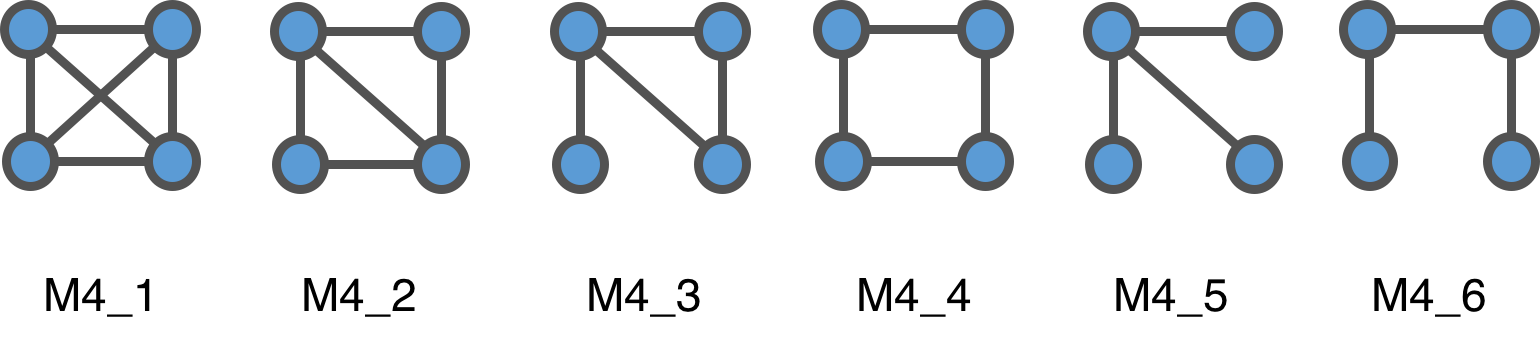
\includegraphics[clip,width=12cm,height = 3cm]{figs/motifs.png}
		\vspace{0.5cm}
		\caption{Network motifs of $k =4$, where $k$ is the number of node in a connected sub-graph.}
		\label{motifs}
	\end{center}
\end{figure}

In order to quantify network motifs, we first count the occurrence of each sub-graph in the original network, then repeat the same process on the randomized networks that have the exact same degree distribution. Such random networks are often referred to as \textit{configuration model} and are widely used as a null model for calculating various statistics related to networks. After counting occurrences of sub-graphs in both original and multiple random networks, we proceed to calculate z-score for each sub-graph $i$ as follows:
	\begin{equation}
	Z_i = \cfrac{N_i^{\text{original}} - \langle N_i^{\text{random}} \rangle }{\sigma_i^{\text{random}}},
	\end{equation}

where $N_i^{\text{original}}$ is the number of occurrence of a sub-graph $i$ in the original network and $ \langle N_i^{\text{random}} \rangle$ and $\sigma_i^{\text{random}}$ are the average and the standard deviation of the number of occurrence of a sub-graph $i$ in an ensemble of random networks. It is usually convenient to normalize this z-score as some networks exhibits very large values due to the size of the networks. Such normalized z-score is called \textit{significance profile} and is defined as follows:
	\begin{equation}
	SP_i = \cfrac{Z_i}{\sum_j Z_j^2}.
	\end{equation}
	
In this study, we treat the significance profile for each subgraph as a feature and in total we have six features as network motifs.
\newline



\begin{table}[htb]
  \begin{center}
    \caption{Network Features. The total number of features is $8$.}
    \begin{tabular}{| l | p{8cm} |} \hline
      Name of the feature & Explanation  \\ \hline \hline
      Clustering coefficient &  The probability that a connected triplet ($k=3$ subgraph) is a triangle \\  \hline
      Degree assortativity &  Correlation between a pair of connected nodes' degree. \\  \hline
      Network motifs from $m4\_1$ to  $m4\_6$& The normalized z score of a subgraph's frequency compared to that of an ensemble of random networks having the exact same degree distribution. \\ \hline
    \end{tabular}
    \label{tab:feature}
  \end{center}
\end{table}

%%%%%%%%%%%%%%%% --- New Chapter --- %%%%%%%%%%%%%%%%
\newpage
\section{Data Sets}
	\subsection{Description}	
	Our network data set has been accumulated with a lot of effort over years and hyperlinks to most of the data are available at the website of The Colorado Index of Complex Networks (ICON) \url{https://icon.colorado.edu}. ICON is essentially the place where hyperlinks to the network data are stored, rather than the data itself.  
	Since data format of real world networks is not standardized, we proceeded to convert all the data into a single format called \textit{Graph Modeling Language} or simply GML \cite{GML}. The format allows us to flexibly specify arbitrary node and edge attributes. We, however, do not use any node and edge attribute, including edge weight, as well as edge directionality at all since not all of networks have such properties and we wanted to analyze a diverse set of networks. Thus, we treat all networks used in this study as a simple graph which is defined in the previous chapter. We have used only a fraction of all networks available on ICON due to the time constraint. We have also added some synthesized network data which are generated from specific models as follows: 1. Erd\H{o}s-R\'enyi random network (ER Network) \cite{ER_Network}, Watts-Strogatz model (Small World) \cite{watts1998cds}, Barab\'asi-Albert model (Scale Free) \cite{Barabasi99emergenceScaling} and the forest fire model (Forest Fire Network) \cite{ForestFire}. The details of network sub-domains are explained in the table \ref{tab:subdomain}.
	
	The distributions of network domains and sub-domains, as shown in figs.\ref{domain_ratio} and \ref{sub_dist}, are very skewed since instances of some network categories are hard to obtain due to their inherent difficulty of collecting data or legal concerns, or hard to analyze due to their network size. This skewed categorical distribution leads us to explore several sampling methods, which are explained in the following chapter. 
	\subsection{Feature Extraction}
	After converting into GML format, we calculate a set of features explained in the previous chapter for each network. We have extensively used a Python library \textit{igraph} \cite{igraph} for extracting features including clustering coefficient and degree assortativity and other miscellaneous operations on network data. For calculating network motifs, we used a parallel motif computing algorithm for undirected motifs developed by Ahmed \textit{et al.} \cite{ahmed2015icdm}. A number of computations involved in this study are parallelized by using a command-line tool \textit{GNU Parallel} \cite{GNUParallel}.

\begin{figure}[H]
\begin{subfigure}{0.40\textwidth}
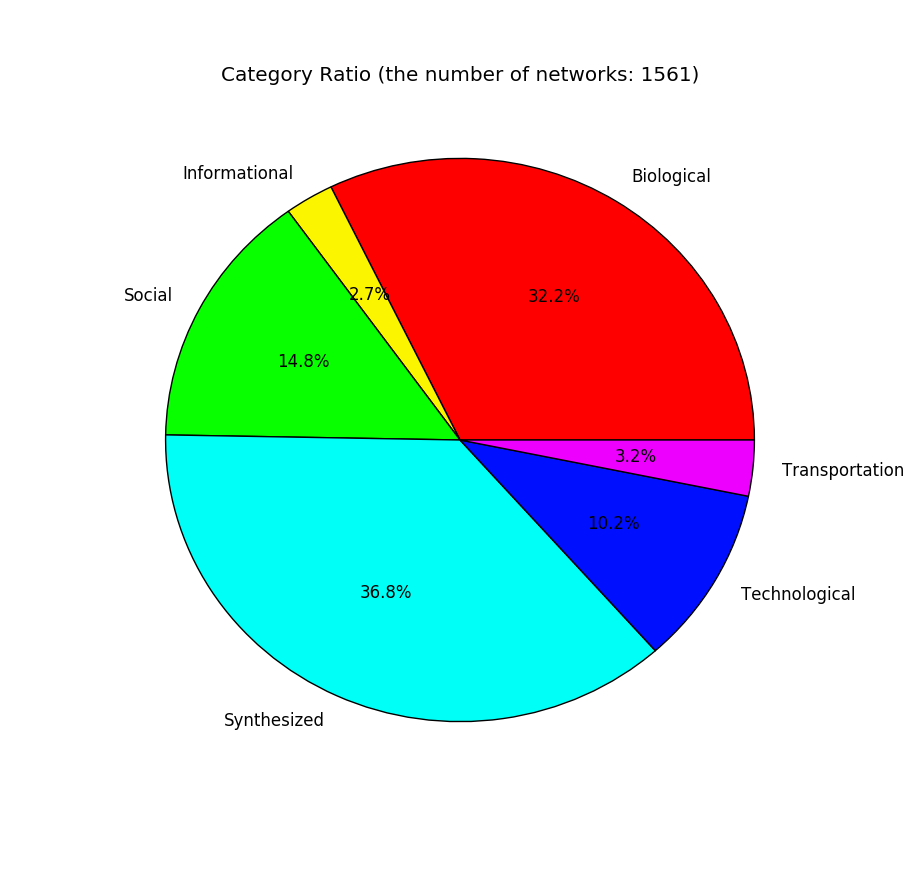
\includegraphics[width=\linewidth]{figs/category_ratio.png}
\caption{}\label{domain_ratio}
\end{subfigure}\hspace*{\fill}
\begin{subfigure}{0.45\textwidth}
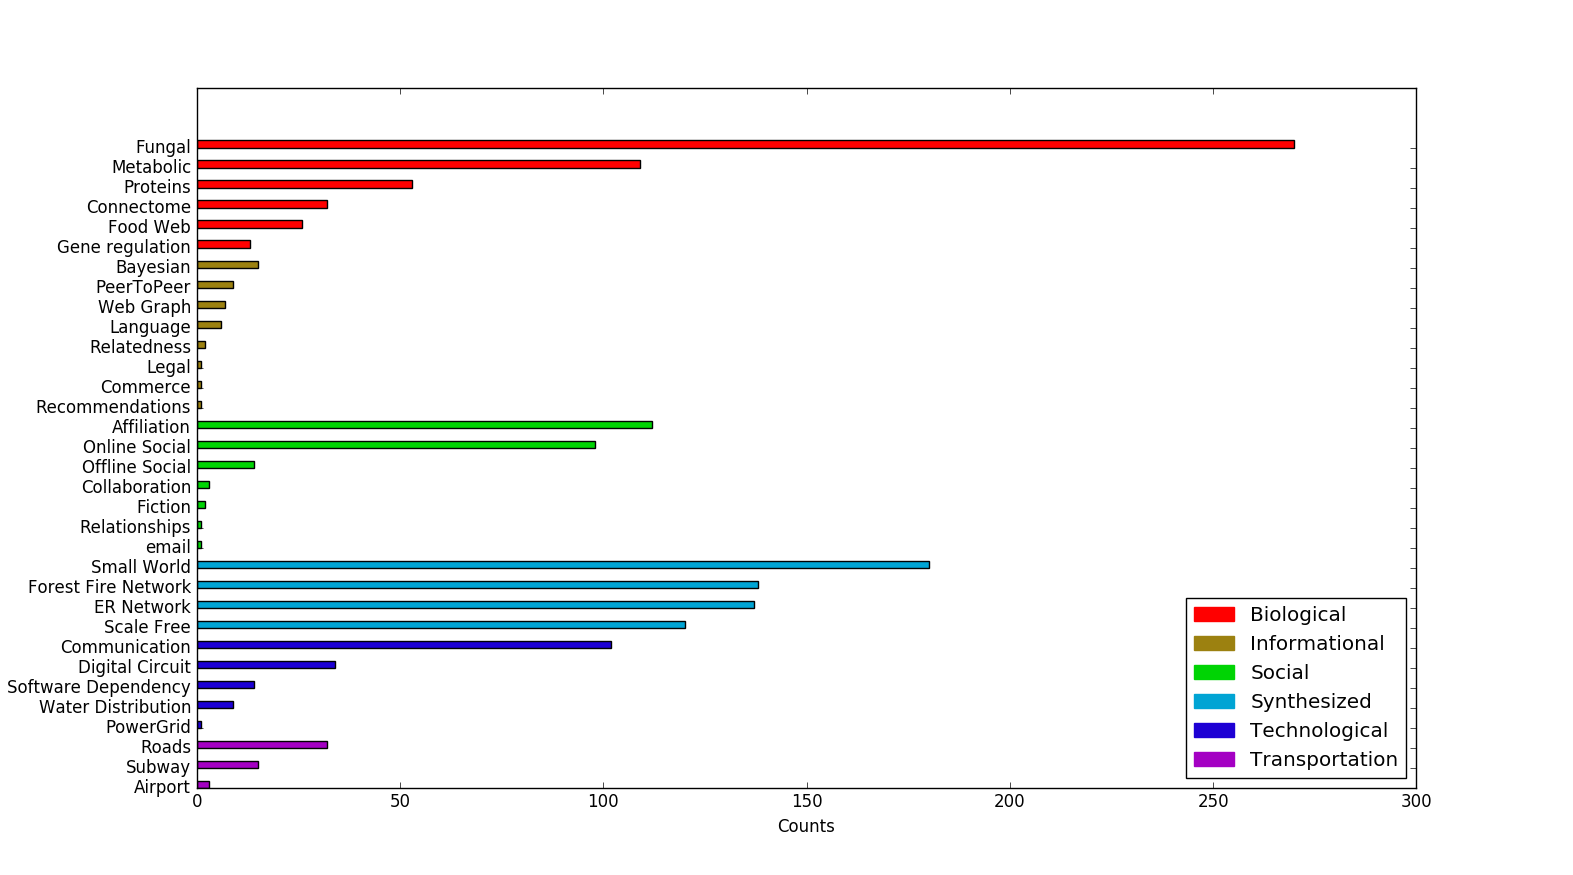
\includegraphics[width=\linewidth]{figs/subdomain_dist.png}
\caption{}\label{sub_dist}
\end{subfigure}\hspace*{\fill}

\caption{(a): The categorical ratio of network domains. (b):  Count distribution of network sub-domains. Sub-domains of the same network domain are grouped together having the same color in the figure. Color code from top: Biological, Informational, Social, Synthesized, Technological and Transportation.} \label{category_dist}.
\end{figure}


\newpage
	\begin{longtable}{| l | l | p{9cm} |}
	\caption{Network sub-domains and their descriptions.} \label{tab:subdomain}\\
	
	%header for the first page%
	\hline
 	Sub-domain & Domain& Description \\ \hline \hline
	 \endfirsthead
	 % header for after the first page
	 \multicolumn{3}{l}{\small\it Continued}\\ \hline
	 Sub-domain & Domain& Description \\ \hline \hline
 	\endhead
      %Sub-domain & Domain & Description  \\ \hline \hline
      Fungal &  Biological & Network of mycelial growth patterns of fungus or slime mold. Nodes are located at hyphal tips, branch points, and anastomoses. Edges represent cords.\\  \hline
      Metabolic &  Biological & Network of chemical reactions of metabolism in a cell.\\  \hline
      Proteins &  Biological & Physical contacts of proteins in a cell or in a living organism.\\  \hline
      Connectome &  Biological & Network of neural connection in the brain at either the level of neuron or the level of anatomical region.\\  \hline
      Food Web &  Biological & The relationships of predator-prey in terrestrial or aquatic animal kingdoms.\\  \hline
      Gene regulation &  Biological & The interactions of molecular regulators that govern the gene expression.\\  \hline
      Bayesian & Informational & Probabilistic model that contains a directed-acyclic-graph(DAG) in which nodes represent random variables and edges represent conditional dependence among these random variables.\\  \hline
      PeerToPeer &  Informational & A kind of computer networks in which peers (computers) are equally privileged in the network for sharing files.\\  \hline
      Web Graph &  Informational & Network of World-Wide-Web. Nodes represent web pages and edges represent hyper-links among web sites. \\  \hline
      Language &  Informational & Networks of word adjacency and word association.\\  \hline
      Relatedness &  Informational & Networks of relatedness, such as similarities among book purchased on online retailers. \\  \hline
      Legal &  Informational & Network of legal citations. Nodes represent majority opinions written by the Supreme Court of the United States and edges represent citation.\\  \hline
      Commerce &  Informational & Network of co-purchasing items on websites.\\  \hline
      Recommendations &  Informational & Network of books, where edges represent the frequency that a pair of nodes (books) is co-purchased together.\\  \hline
      Affiliation &  Social & Network of cooperate board members. Networks in this sub-domain are one-mode projected onto individuals.\\  \hline
      Online Social &  Social & Network of friendship online, such as Facebook.\\  \hline
      Offline Social &  Social & Network of friendship or some sort of inter-personal relationships offline.\\  \hline
      Collaboration &  Social & Network of collaborations among people. This sub-domain includes collaboration of scientific papers, music, etc.\\  \hline
      Fiction &  Social & Co-appearance network of fictional characters from books.\\  \hline
      Relationships &  Social & Network of social relationship among managers from tech companies, Florentine families during the Italian Renaissance, etc.\\  \hline
      Email &  Social & Network of emails.\\  \hline
      Small World &  Synthesized & Networks generated by Watt-Strogatz model.\\  \hline
      Forest Fire Network &  Synthesized & Networks generated by a Forest Fire Model proposed by Leskovec \textit{et al.} \\  \hline
      ER Network &  Synthesized & Erd\H{o}s-R\'enyi random network. \\  \hline
      Scale Free &  Synthesized & Networks generated by Barab\'asi-Albert model.\\  \hline
      Communication &  Technological & Network of autonomous systems (the Internet).\\  \hline
      Digital Circuit &  Technological & Networks of logical gates connected by wirings.\\  \hline
      Software Dependency &  Technological & Networks in which nodes represent either class, function or package and edges correspond to dependencies.\\  \hline
      Water Distribution &  Technological & Network of piping and junctions for water distribution system.\\  \hline
      Power Grid &  Technological & Network of power grid in which nodes correspond to transforms or power relay points and edges represent power lines.\\  \hline
      Roads &  Transportation & Network of roads where nodes are intersections and edges are roads.\\  \hline
      Subway &  Transportation & Subway networks of major cities around the world.\\  \hline
      Airport &  Transportation & Network of airports that are connected by flights between the airports.\\  \hline
           
\end{longtable}


%%%%%%%%%%%%%%%% --- New Chapter --- %%%%%%%%%%%%%%%%
\newpage
\section{Methodology}
After having converted networks into vectors in the feature space, there are a number of possible ways to analyze the distribution of points and labels and possibly learn the concept that governs such distribution in the feature space. In this study, we use random forest classifier along with the confusion matrix as a way to learn the underlying concept that differentiates different classes of networks. As we have seen in the previous chapter, the distribution of class labels is obviously skewed which leads us to use several sampling methods that are supposed to alleviate the problem. In this chapter, we explain such methodologies in the great detail.

	\subsection{Sampling Methods}
Most of machine learning algorithms perform well on evenly populated instances of multiple classes. However, once this class balance no longer persists, the algorithms perform poorly on minority classes. This problem, called \textit{class imbalance}, essentially causes any machine learning algorithm that is naive to the data set to focus exclusively on the majority class, ignoring any minority classes. One of the most widely used approaches for mitigating the problem is sampling the data set of interest so that the distribution of classes becomes balanced. Although there are many proposed sampling strategies as of now \cite{SurveySampling}, we primarily use three sampling strategies in this study: random over-sampling, random under-sampling and SMOTE \cite{SMOTE}.

 Here we establish the mathematical notations used in explaining sampling methods. Let $S$ be a set of pairs of $\vec{x_i}$ and $y_i$, namely $S =\{(\vec{x_i},y_i)\}, i = 1,...,n$ where $n$ is the number of data, $\vec{x_i} \in X$ is an instance of networks in the $N$-dimensional feature space and $y_i \in Y = \{1,...,C\}$ is a class label associated with the instance $\vec{x_i}$.   


		\subsubsection{Random Over-sampling}
		Random sampling method is one of the simplest strategies for mitigating the class imbalance problem. \textit{Random over-sampling} essentially over-samples any minority classes to an extent that the number of instances in each class becomes even. Here we explain this sampling method in a mathematical sense. Let $S_{maj} \subset S$ be the majority class, meaning a class having the largest number of instances, and $S_{min}^{j}$ be the $j$th minority class where $j = 1,...,C-1$ such that
	
	
	\begin{equation}
	S_{maj} \cap S_{min}^{1} \cap S_{min}^{2},..., \cap S_{min}^{C-1} = \{\},
	\end{equation}
	and
	\begin{equation}
	S_{maj} \cup S_{min}^{1} \cup S_{min}^{2},..., \cup S_{min}^{C-1} = S.
	\end{equation}
	
	
Let $E_{min}^j$ be a set of points that are sampled at uniformly random from a set $S_{min}^{j}$ that satisfies the following equality:

	\begin{equation}
	|S_{min}^{j}| + | E_{min}^j | = |S_{maj}|.
	\end{equation}
	
 We then append the set $E_{min}^j$ to the corresponding set of the minority class $S_{min}^{j}$, namely $S_{min}^{j} := S_{min}^{j} + E_{min}^j$. The drawback of random over-sampling is a potential poor generalization due to the overfit of a classifier to the over-sampled instances.
	
	\subsubsection{Random Under-sampling}
	\textit{Random under-sampling}, on the other hand, under-samples the majority class, essentially throwing out some data in order to make the "cloud" of data points sparser. This "throwing out instances" implies an obvious drawback of this sampling method: It discards potentially important instances that compose the backbone of majority classes, implying the true shape of majority class is no longer retained. Here, again, we explain this method using mathematics. Let $S_{min} \subset S$ be the minority class,
meaning a class having the least number of instances, and  $S_{maj}^{j}$ be the $j$th majority class where $j = 1,...,C-1$, such that

	\begin{equation}
	S_{min} \cap S_{maj}^{1} \cap S_{maj}^{2},..., \cap S_{maj}^{C-1} = \{\},
	\end{equation}
	and
	\begin{equation}
	S_{min} \cup S_{maj}^{1} \cup S_{maj}^{2},..., \cup S_{maj}^{C-1} = S.
	\end{equation}
	
Let $E_{maj}^j$ be a set of points that are sampled at uniformly random from a set $S_{maj}^{j}$ that satisfies the following equality:

	\begin{equation}
	|S_{min}^{j}| = | S_{maj}^j -  E_{maj}^j |.
	\end{equation}
Then, we subtract the set $S_{maj}^j$ by $E_{maj}^j$, thus $S_{maj}^j := S_{maj}^j -  E_{maj}^j$.
		
		\subsubsection{SMOTE}
		\textit{Synthetic Minority Over-sampling Technique}, widely known as SMOTE \cite{SMOTE}, is an alternative sampling method that synthesizes data points in the training set for a classifier. Mathematically speaking, SMOTE is quite similar to random over-sampling, except the generation of a set $E_{min}^j$ for a minority class $S_{min}^j$. For each set of the minority class $j$, namely $S_{min}^j$, consider $K$ nearest neighbors of a point $\vec{x_i} \in S_{min}^j$ in the $N$-dimensional feature space. To generate a new point, first pick up one of the $K$ nearest neighbors, say $\vec{x_{n}}$, then multiply the corresponding feature vector difference with a weight  $\delta$  chosen from an interval $ [0,1]$ at uniformly random and add this vector to $\vec{x_i}$. Therefore, we have a newly synthesized point defined as follows:
		
		\begin{equation}
		\vec{x_{new}} = \vec{x_{i}} + \delta*(\vec{x_{n}} - \vec{x_{i}}).
		\end{equation}

And one repeats this procedure for other neighbors of the point $\vec{x_i}$ and construct a set $E_{min}^j$. See the figure \ref{smote} for visualization the process synthesizing.	
		
		\begin{figure}[ht]
		\begin{center}
		\vspace{0.5cm}
		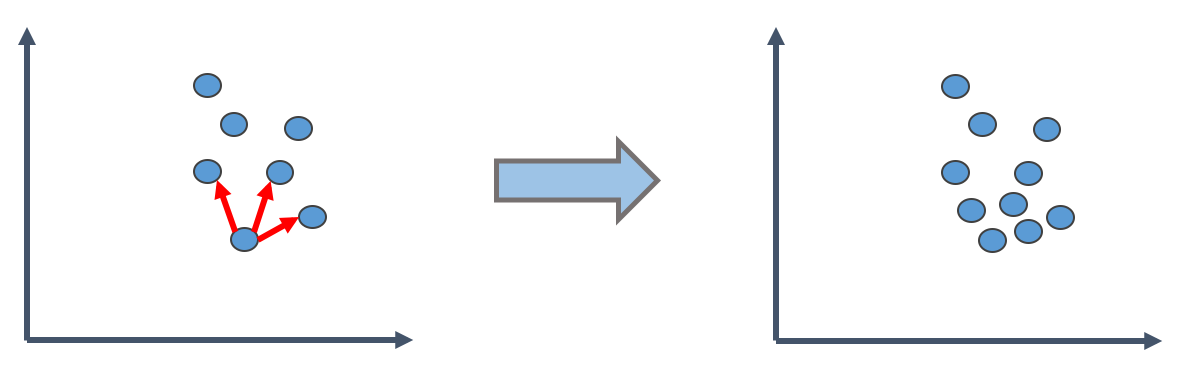
\includegraphics[clip,width=12cm,height = 3cm]{figs/SMOTE.png}
		\vspace{0.5cm}
		\caption{Synthesizing phase of SMOTE. Here the number of nearest neighbors $k$ is 3.}
		\label{smote}
		\end{center}
		\end{figure}
		

The core concept of SMOTE is filling out the cloud of minority class instances by interpolating existing data points so it closely resembles a \textit{convex set}. This idea, making a convex set of minority instances by interpolation, assumes that the underling data distribution itself is convex. In a high dimensional space, it is often the case that the distribution of data forms a quite intricate manifold from which the data we observe is generated. So interpolating data points of the complex manifold yields a convex set, that is radically different from the underlying concept that a classifier tries to learn.

	\subsection{Classification}
	In order to find similarities and differences of data of different classes, one needs to develop a notion of "distance" between the classes. In this study we derive such notion of distance from confusion matrices that are produced by random forest classifiers. Following sub-sections describe the details of decision tree which is an essential component of random forest, random forest classifier and confusion matrix.
	
		\subsubsection{Decision Tree}
		Decision tree is a model which describes the relationship between input variables and output class by recursively asking a question on a single input variable and splitting the data set into two based on the answer to the question until a data set has enough homogeneity of a class in it. In a high dimensional space, such spitting the data set corresponds to hyperplane in the space. The algorithm for learning decision tree splits the data set based on a criterion of values of an input variable such that the resulting data sets become less heterogeneous or less "impure" in terms of class labels. One of the widely used such criteria and the one we use in this study is \textit{Gini impurity}. The definition of Gini impurity for a data set with $J$ classes is the following:
	\begin{equation}
	I_G(f) = \sum_{i=1}^J f_i(1-f_i) = \sum_{i=1}^J (f_i-f_i^2) =  \sum_{i=1}^J f_i - \sum_{i=1}^J f_i^2 = 1- \sum_{i=1}^J f_i^2,
	\end{equation}
where $f_i$ is a probability that an item that belongs to class $i$ is chosen in the data set. Gini impurity becomes $0$ if all items in a set belong to the same class, meaning the set is "pure" and takes a value greater than $0$ if the set contains items of multiple classes. Each splitting essentially seeks the best possible value of an input variable such that the decrease of Gini impurity is the largest when the data set is split at the value (or hyperplane defined with it). Splitting continues until no further improvement can be made and the terminal of a tree are called leaves of the tree, each corresponding to one of the class labels in the data set.
		
	
		\subsubsection{Random Forest Classifier}
Random forest is a type of \textit{ensemble learning method} that combines a number of so called "weak" classifiers together \cite{RandomForest}. When it's given a data set to predict after training weak classifiers, it outputs a majority of all outputs from the weak classifiers and this aggregation of weak classifiers prevents random forest from overfitting to the training data. In random forest, such weak classifiers are decision tree which is explained in the previous section.

The learning phase of random forest classifier first involves random sub-sampling of the original data with replacement for $B$ times, each time the sub-sampled data set is fed to a decision tree. For each decision tree a set of randomly sampled input variables (features) is used for splitting and this randomly selecting features is called random subspace method or feature bagging. This prevents the classifier to focus too much on feature sets that are highly predictive in the training set. 

One of the advantageous byproducts of random forest is that one could rank input variables or features based on the importance in the classification. Each time a split is made on a node in a decision tree, the decease of Gini impurity can be attributed to selecting a feature as a splitting point.  Calculating the average decrease of Gini impurity for selecting a feature over all decision trees in random forest gives us the importance of the feature that is very consistent with the result of original method for calculating variable importance \cite{RandomForest,RandomForestOnline}. This ranking of feature importance is the crucial part of the analysis we we describe in the next chapter.


		\subsubsection{Confusion Matrix and Similarity}
	Confusion matrix depicts when and how frequently a classifier makes mistakes. The row labels of the matrix usually correspond to  true labels and column labels correspond to predicted labels. An element $c_{ij}$ in a confusion matrix represents the number of occurrences that a classifier predicted an instance of class $i$ as class $j$. So it is easy to notice that diagonal elements of a confusion matrix, namely $c_{ii}$ for $i = 1,...,n$ represents the correct predictions of a classifier. What we are interested in, however, lies in off-diagonal elements of a confusion matrix. The information that a classifier gets confused with classes $i$ and $j$ implies the similarity or distance between classes: if the points of two different classes in a high dimensional feature space are often misclassified as each other,  
the points of the two classes are in fact overlapped to some extent in the feature space, implying that these classes are so similar the distance between them is small.

Using a confusion matrix as a similarity matrix involves following issues:
\begin{enumerate}
	\item In a confusion matrix classes with abundant data tend to have large counts for elements in the matrix due to the abundance of test data whereas classes with fewer data have fewer counts in the matrix.
	\item Usually the confusion matrix is not symmetrical, but a number of similarity-related methods assume an input matrix has the symmetry.
\end{enumerate}

Therefore we proceed on the following operations in order to derive a similarity matrix based on a confusion matrix:
\begin{enumerate}
	\item Normalize each row $i$ of the confusion matrix so that $\sum_{j=1}^J c_{ij} = 1$
	\item Symmetrize the resulting matrix from operation $1$ by setting each pair of symmetric elements as: $c_{ij},c_{ji} = \max (c_{ij},c_{ji})$
\end{enumerate}

We utilize the similarity matrix produced in this way in experiments which are described in the subsequent chapter.

%%%%%%%%%%%%%%%% --- New Chapter --- %%%%%%%%%%%%%%%%
\newpage	
\section{Analyses}
In this chapter, we present experimental settings for analyses, each of which tries to gain some insights for answering the questions we proposed in the introduction, and show the results of such analyses.
\subsection{Discriminative Feature Set}
The first question we have asked was: \textit{What aspects of network structure do make a specific category of network different from others?} This question can be answered by looking at the statistics of feature importance from random forest classifiers. The experimental setting is the following: 

\begin{enumerate}
	\item We select a set of six representative network sub-domains since not all of the sub-domains have enough number of samples to support our findings. These representative sub-domains are: protein interaction, ecological food web, metabolic, connectome (brain networks),  online social and communication (autonomous systems).
	\item For each representative class we proceed to run binary classification 1000 times using random forest in which all of the class labels are grouped together except the target class label. A set of features for this task includes: clustering coefficient, degree assortativity and $k = 4$ connected network motifs, thus the total of eight features. In each run we split the data set into training and test sets with the ratio of $7:3$ while preserving the ratio of class distribution. In each run the score of accuracy and AUC (Area Under the ROC Curve) is calculated and the ranking of feature importance is recorded. We then average accuracy and AUC scores over 1000 runs and aggregate all of the recorded rankings of feature importance.
	\item Lastly we select the two most important features from the aggregated ranking, plot the all of the data points in the two dimensional feature space in which x and y axes correspond to the most and second most important features, respectively.
\end{enumerate}

Fig.\ref{2d_figures} shows two dimensional plots for representative network sub-domains with axes being the top two important features selected from the statistics of aggregated feature importance shown in figure \ref{feature_importance_figures}. One important observation here is the accuracy of a binary classification does not necessary describe the separability of the target class from other aggregated classes. All of the classifications score more than 97\% which seems quite remarkable. Nevertheless, this is due to the effect of class imbalance as we do not sub/over-sample in this analysis. However, the score of AUC well captures the separability of two classes. 

Fig.\ref{feature_importance_figures} shows the aggregated rankings of feature importance. In this figure, one can observe the general trend of informative feature set and the "strength" of those features in the ranking. For example, the motif $m4\_6$ of metabolic networks and the motif $m4\_1$ of online social networks are the most important features and their strength is quite dominant:  $m4\_6$ of metabolic networks ranks as the first 937 times out of 1000 runs and $m4\_1$ of online social networks ranks as the first 971 times  out of 1000 runs, respectively.

These distinguishing features observed in the figures seem to have some implications for the process in a network. Ecological food-webs display the abundance of $m4\_4$ subgraphs, that are thought to be a major constituent elements in the food-webs as it describes layers of food chain. Animals in the same layer in the food chain do not often prey on each other, but prey on animals in a layer below and they are preyed on by animals in a layer above. Online social networks have an unusual number of $m4\_1$ subgraphs, namely $k = 4$ clique, and this indicates the strong locality of social connections. On the other hand, communication networks exhibit the underrepresented number of  $m4\_1$ subgraphs. This may imply the underlying growing or "construction" mechanism of communication systems: the whole system needs to be connected in order for the Internet to work, but does not need too many connections among autonomous systems as the cost for connections should be lowered.

 

\begin{figure}[H]
\begin{subfigure}{0.48\textwidth}
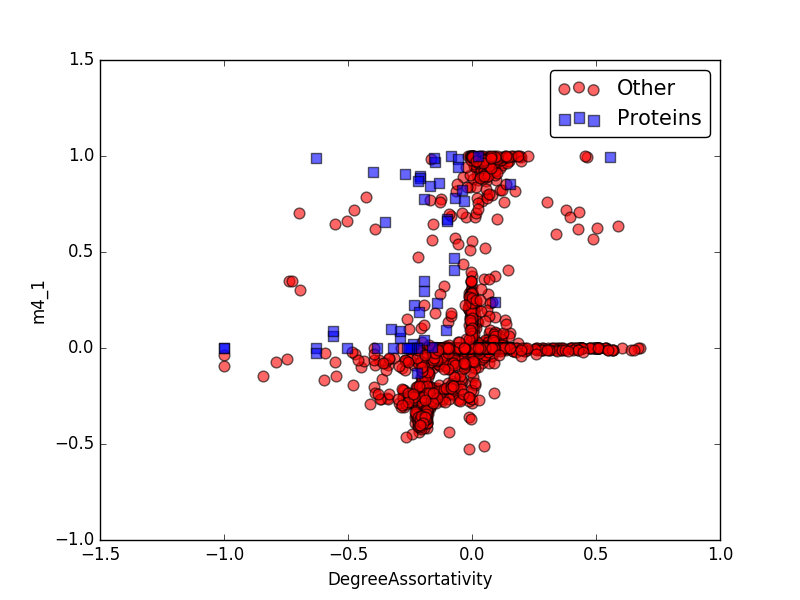
\includegraphics[width=\linewidth]{figs/one_by_many/protein/2d.png}
\caption{Protein interaction. average accuracy: 97.44\%; average AUC score: 0.693} \label{protein_2d}
\end{subfigure}\hspace*{\fill}
\begin{subfigure}{0.48\textwidth}
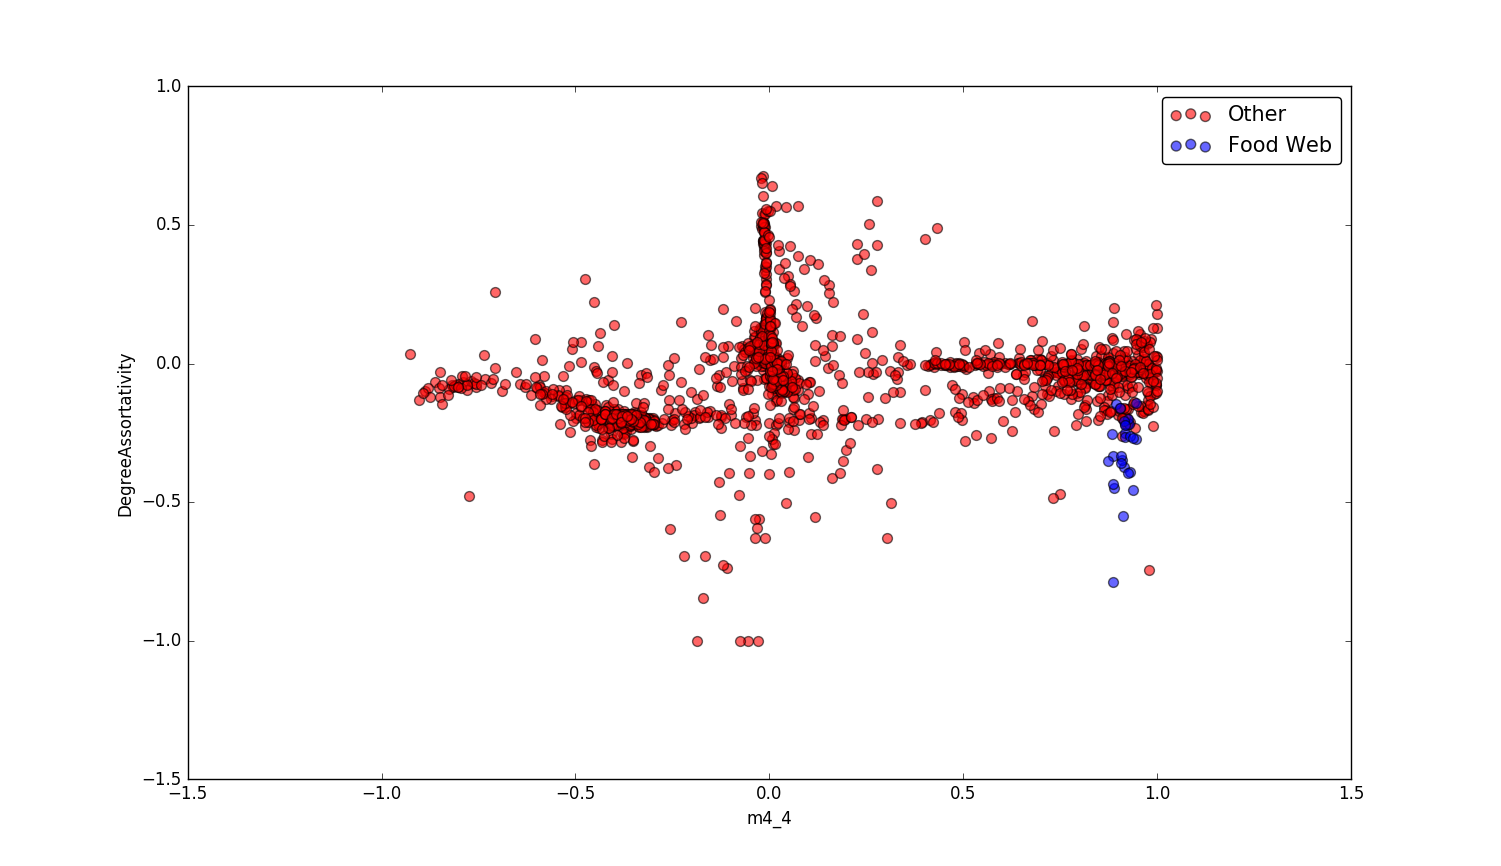
\includegraphics[width=\linewidth]{figs/one_by_many/food_web/2d.png}
\caption{Ecological food web. average accuracy: 99.34\%; average AUC score: 0.802} \label{foodweb_2d}
\end{subfigure}

\medskip
\begin{subfigure}{0.48\textwidth}
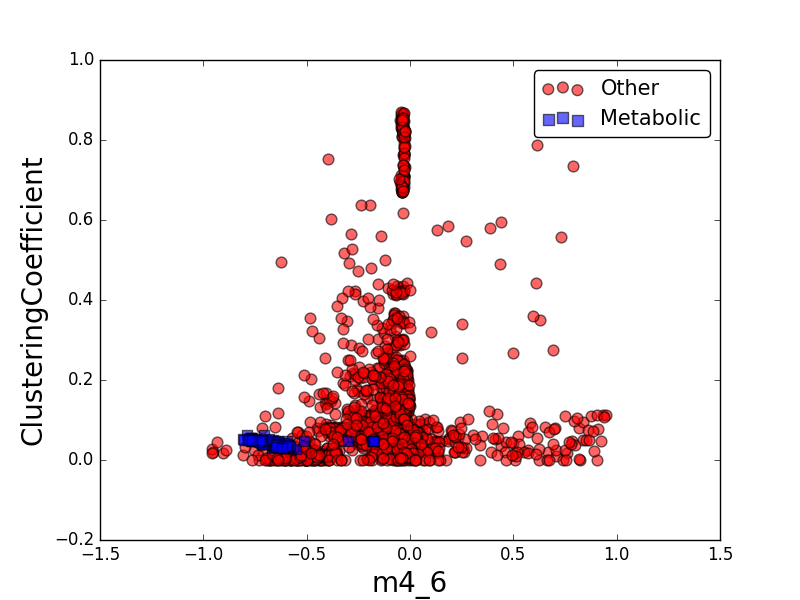
\includegraphics[width=\linewidth]{figs/one_by_many/metabolic/2d.png}
\caption{Metabolic. average accuracy: 99.13\%; average AUC score: 0.94} \label{metabolic_2d}
\end{subfigure}\hspace*{\fill}
\begin{subfigure}{0.48\textwidth}
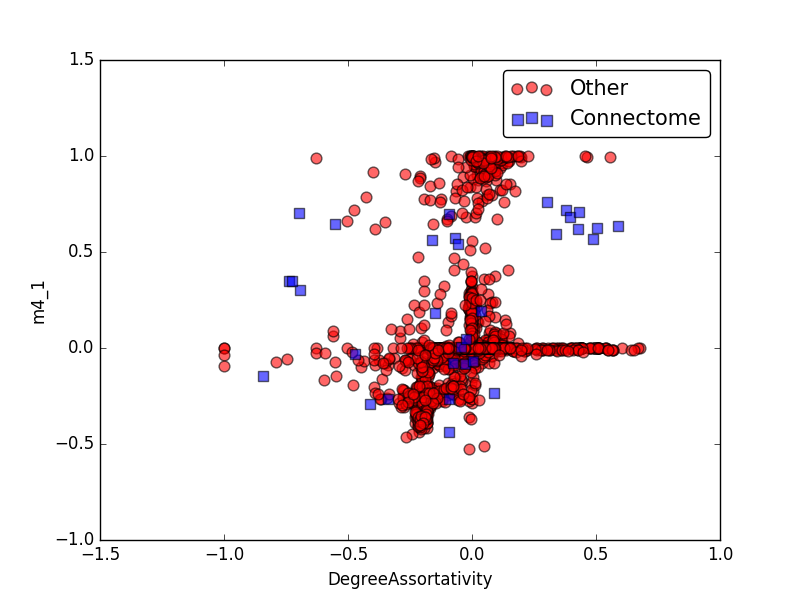
\includegraphics[width=\linewidth]{figs/one_by_many/connectome/2d.png}
\caption{Connectome. average accuracy: 98.8\%; average AUC score: 0.715} \label{connectome_2d}
\end{subfigure}

\medskip
\begin{subfigure}{0.48\textwidth}
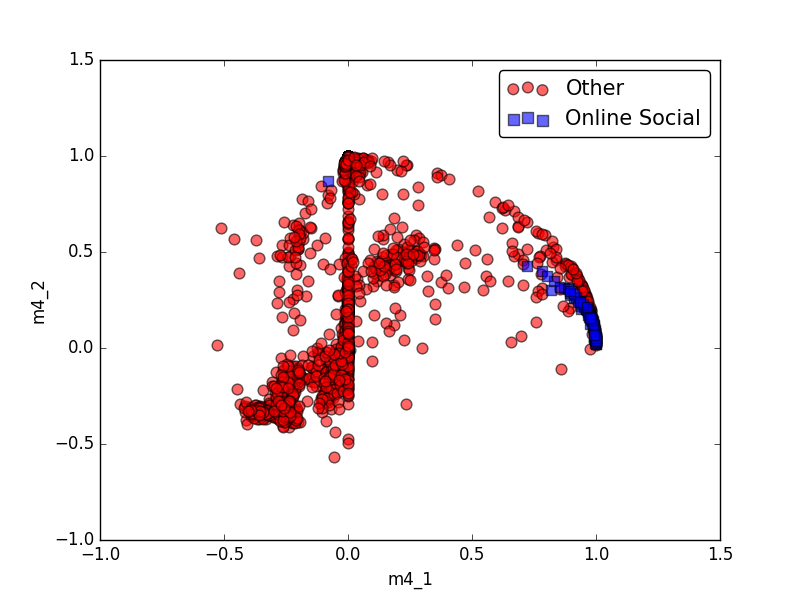
\includegraphics[width=\linewidth]{figs/one_by_many/online_social/2d.png}
\caption{Online social. average accuracy: 99.16\%; average AUC score: 0.939} \label{online_social_2d}
\end{subfigure}\hspace*{\fill}
\begin{subfigure}{0.48\textwidth}
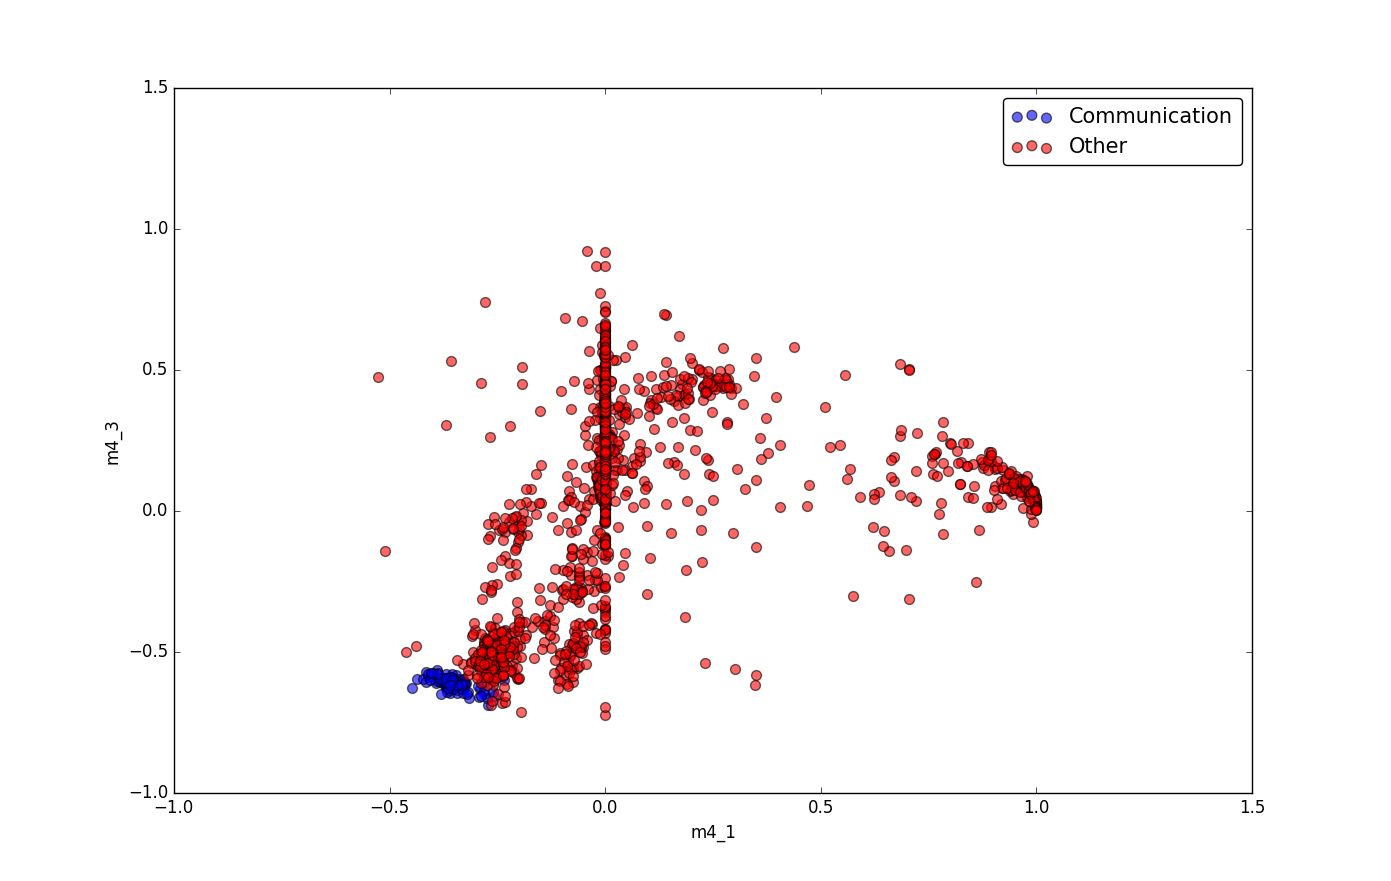
\includegraphics[width=\linewidth]{figs/one_by_many/communication/2d.png}
\caption{Communication. average accuracy: 99.61\%; average AUC score: 0.992} \label{communication_2d}
\end{subfigure}

\caption{2D plots for all representative network sub-domains. X axis corresponds to the most importance feature and y axis the second most important.} \label{2d_figures}
\end{figure}

\begin{figure}[H]
\begin{subfigure}{0.48\textwidth}
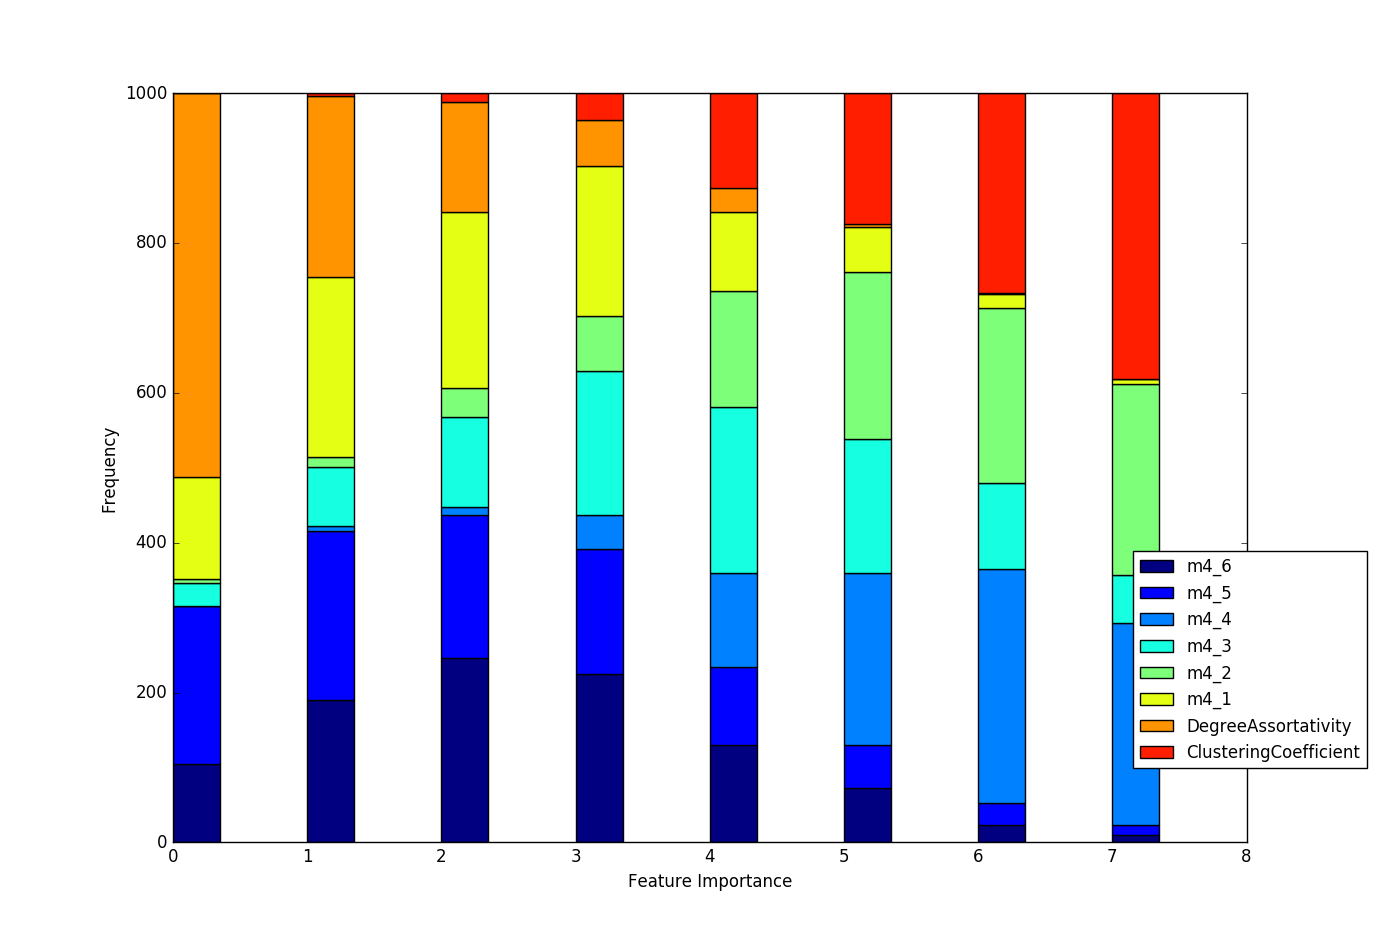
\includegraphics[width=\linewidth]{figs/one_by_many/protein/feature_importance.png}
\caption{Protein interaction.} \label{protein_feature}
\end{subfigure}\hspace*{\fill}
\begin{subfigure}{0.48\textwidth}
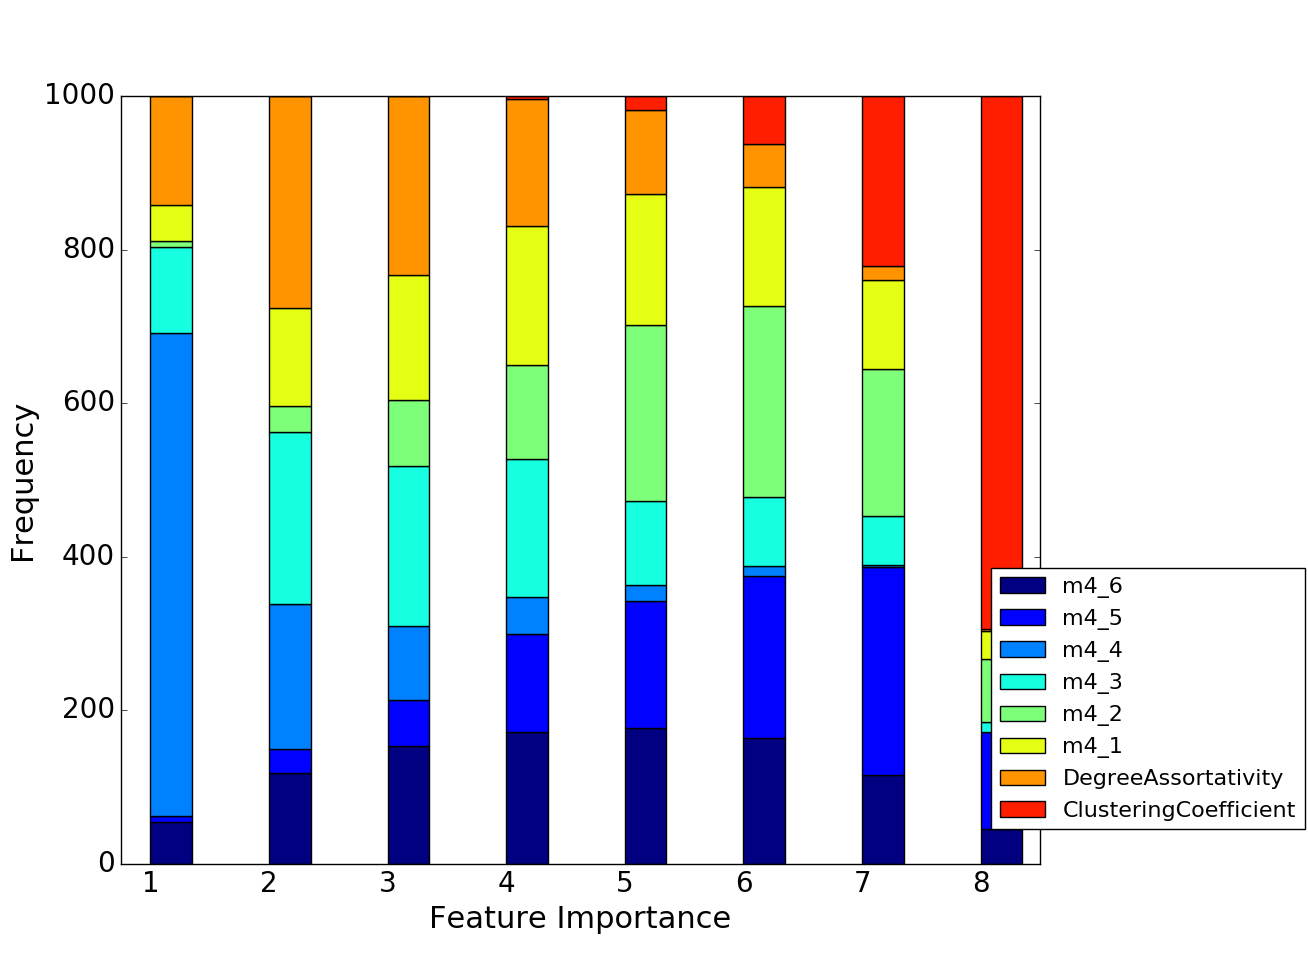
\includegraphics[width=\linewidth]{figs/one_by_many/food_web/feature_importance.png}
\caption{Ecological food web.} \label{foodweb_feature}
\end{subfigure}

\medskip
\begin{subfigure}{0.48\textwidth}
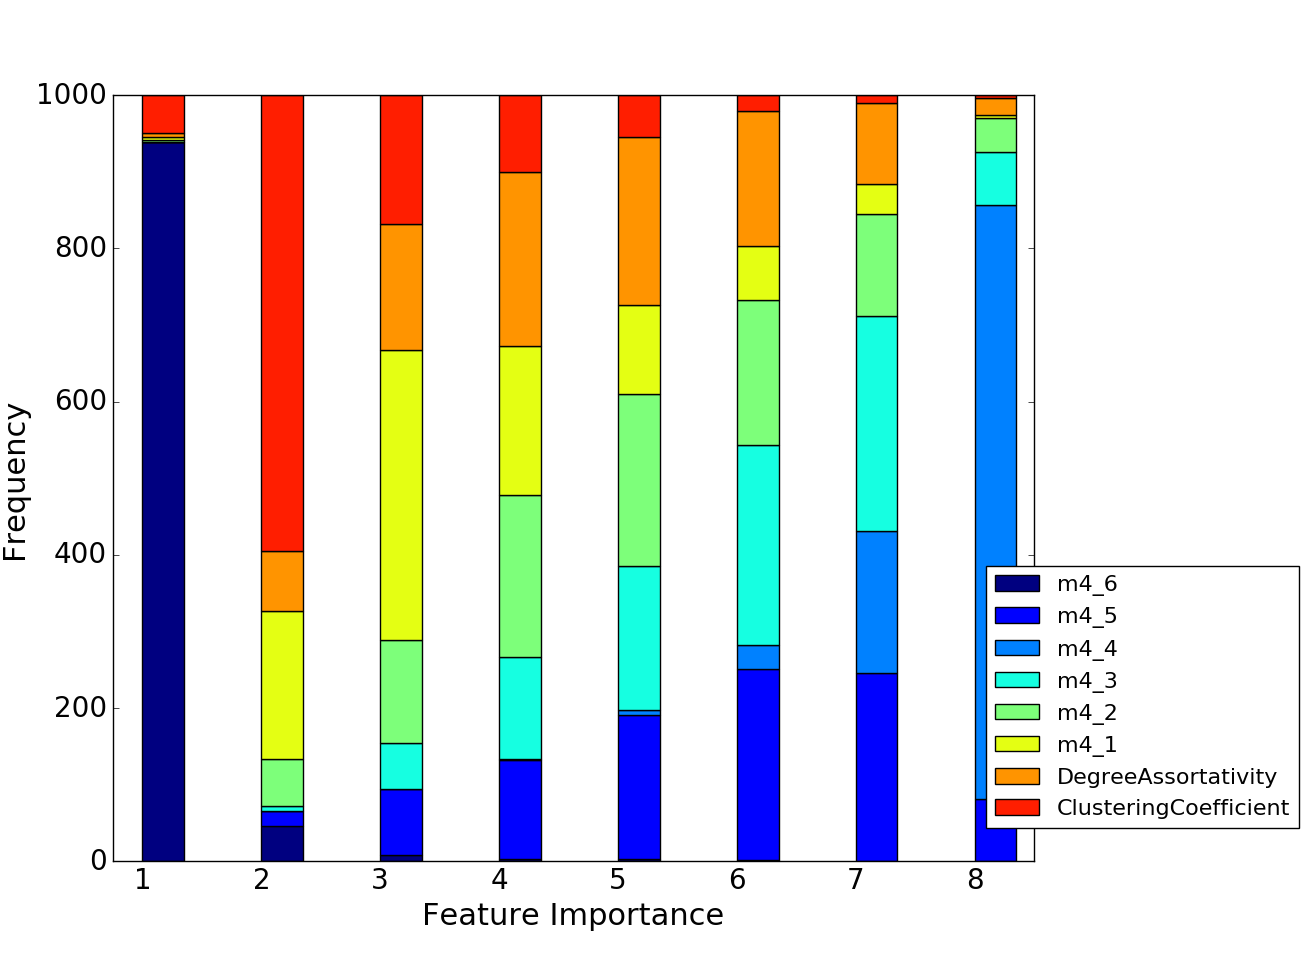
\includegraphics[width=\linewidth]{figs/one_by_many/metabolic/feature_importance.png}
\caption{Metabolic. } \label{metabolic_feature}
\end{subfigure}\hspace*{\fill}
\begin{subfigure}{0.48\textwidth}
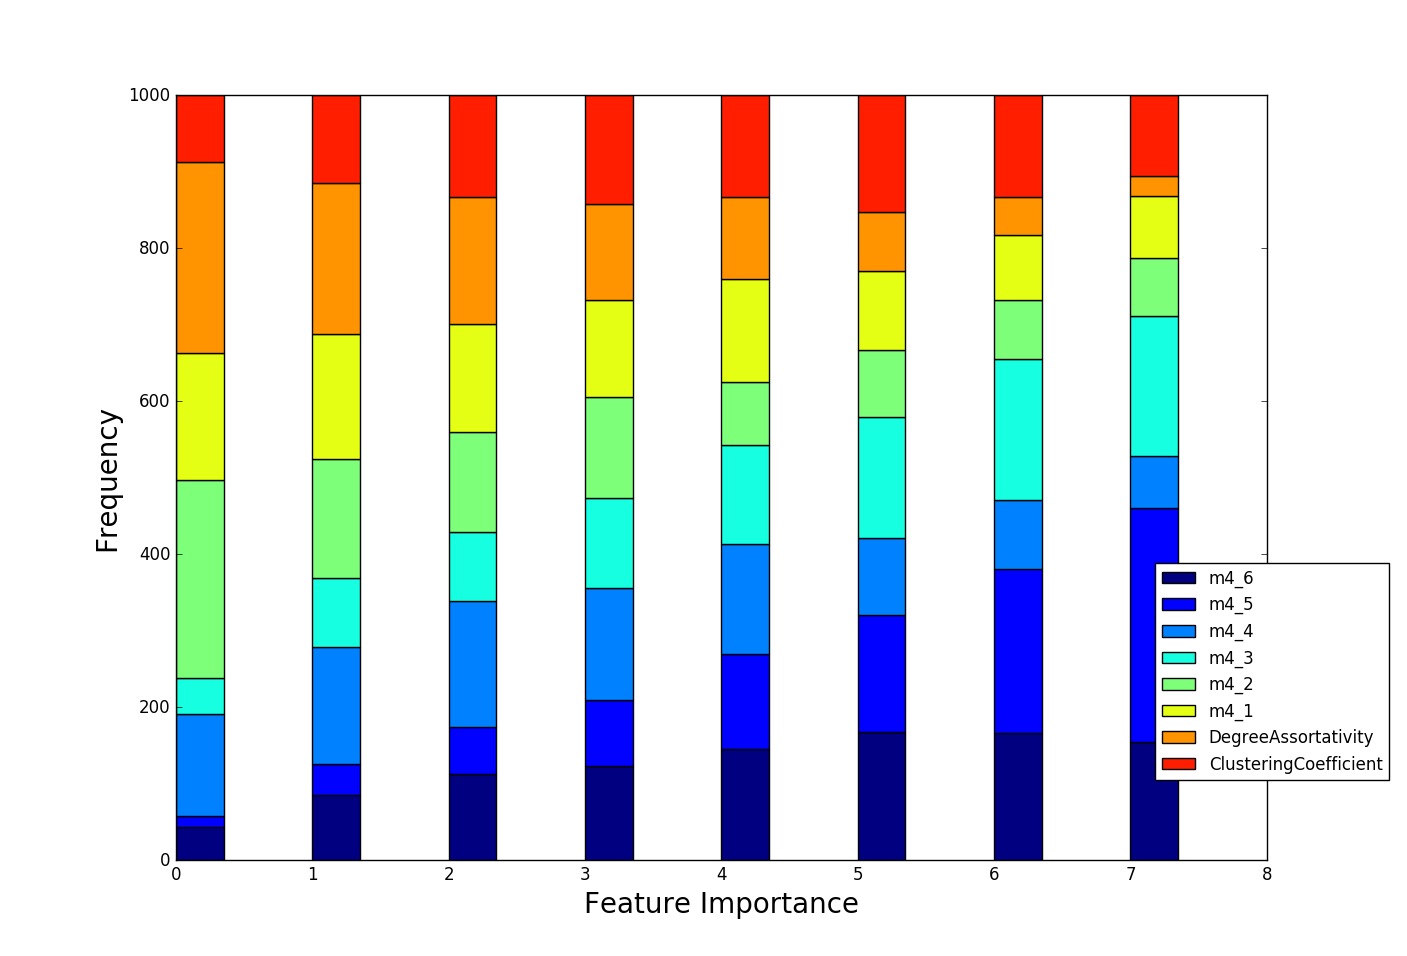
\includegraphics[width=\linewidth]{figs/one_by_many/connectome/feature_importance.png}
\caption{Connectome.} \label{connectome_feature}
\end{subfigure}

\medskip
\begin{subfigure}{0.48\textwidth}
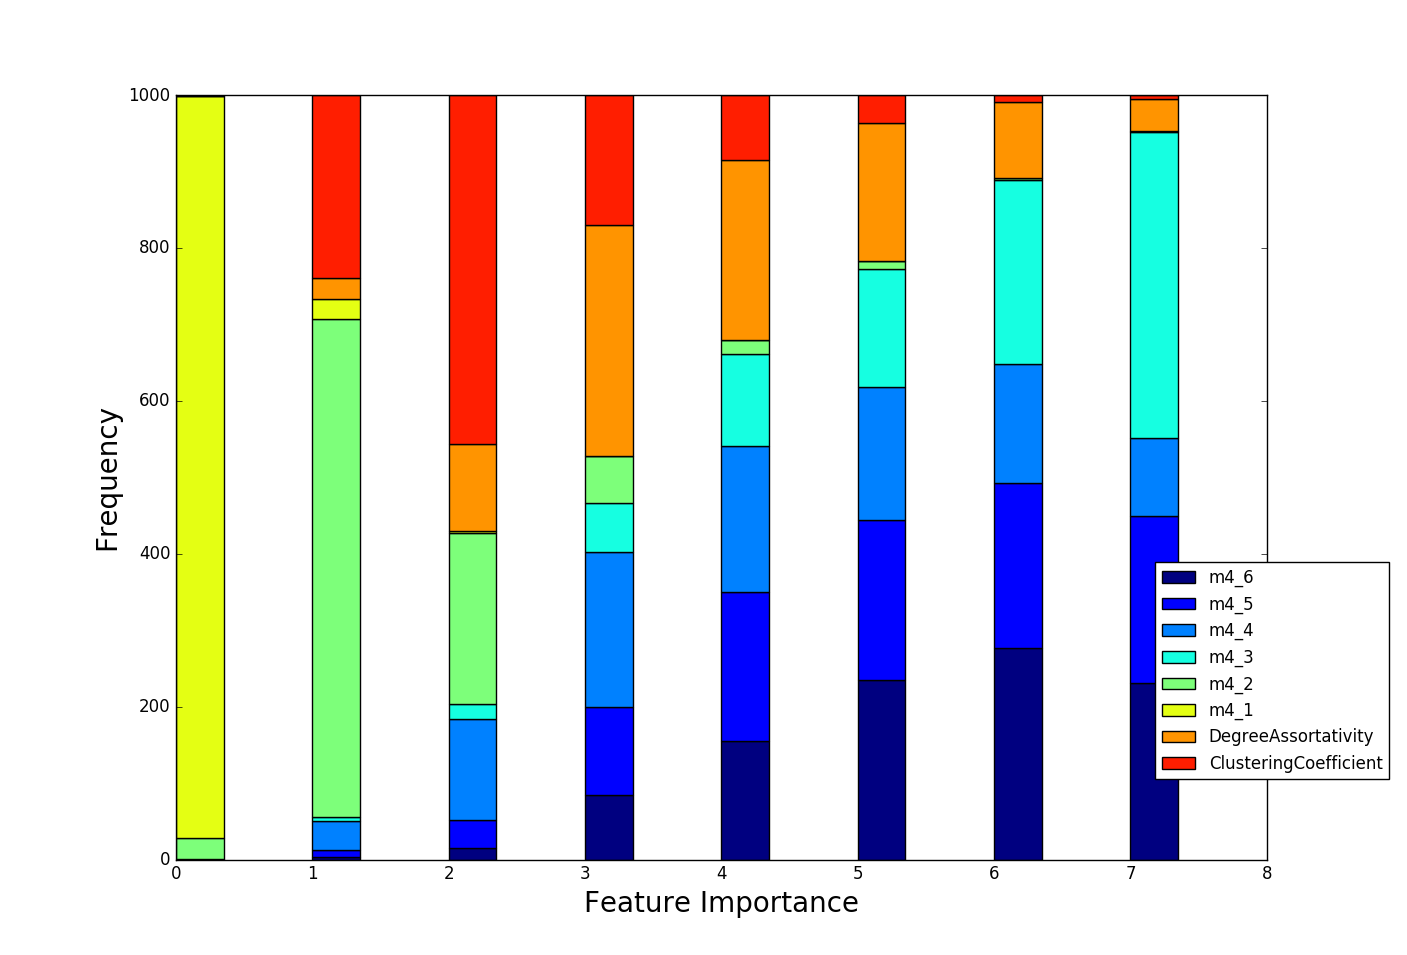
\includegraphics[width=\linewidth]{figs/one_by_many/online_social/feature_importance.png}
\caption{Online social.} \label{online_social_feature}
\end{subfigure}\hspace*{\fill}
\begin{subfigure}{0.48\textwidth}
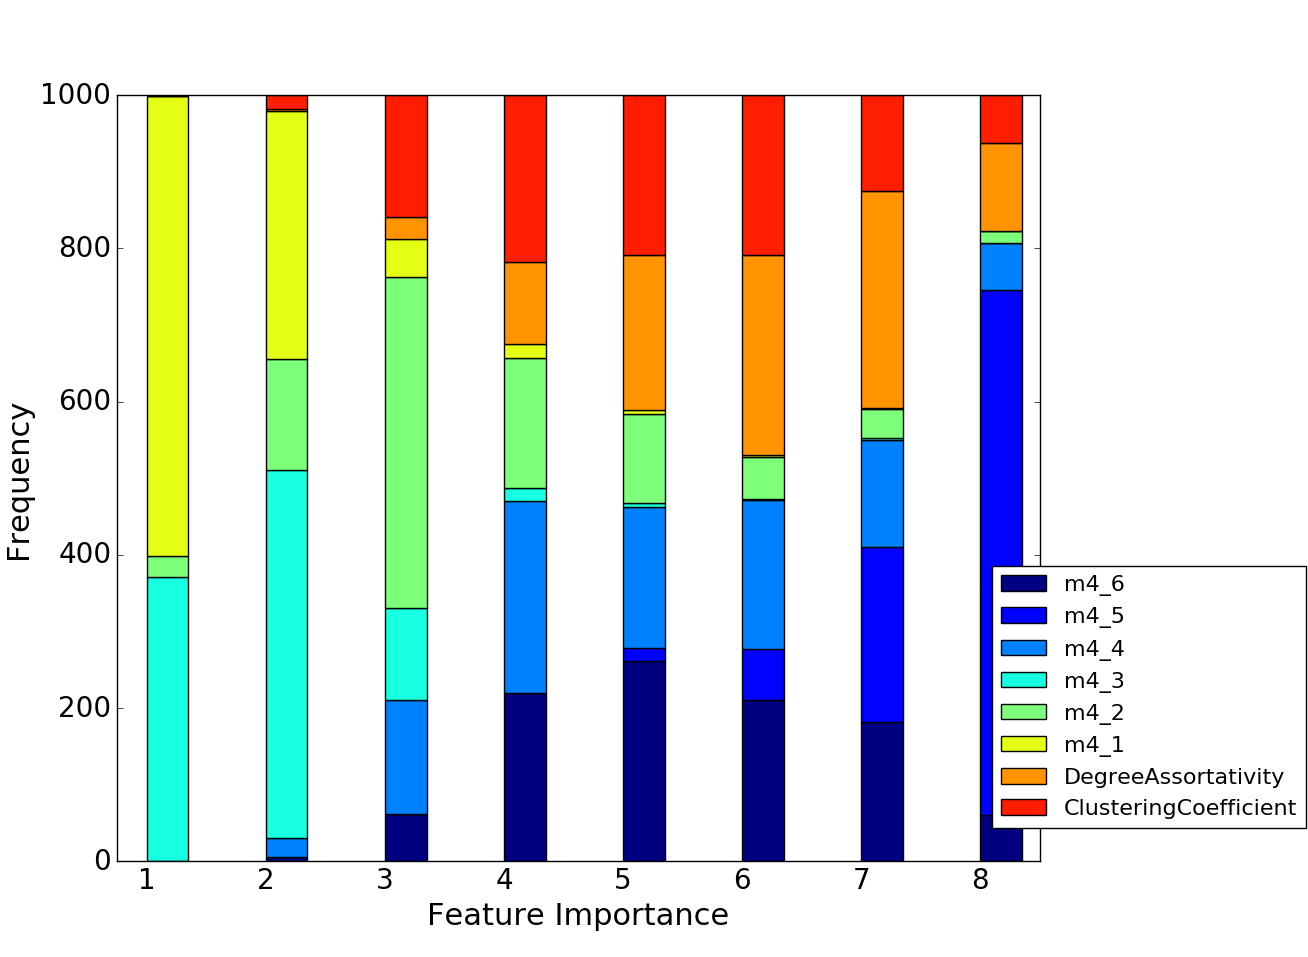
\includegraphics[width=\linewidth]{figs/one_by_many/communication/feature_importance.png}
\caption{Communication.} \label{communication_feature}
\end{subfigure}

\caption{Aggregated rankings of feature importance. The height of a color bar indicates a frequency of the corresponding specific feature being at the rank. The importance decreases along the x-axis} \label{feature_importance_figures}.
\end{figure}


\subsection{Similarities in Networks of Different Kinds}
Every network belongs to some sort of network domain or sub-domain that usually describes the properties and even structure of a network. As we have seen in the previous section, some networks of selected representative sub-domains exhibit structural uniqueness which makes them stand out among others in the feature space. However we can also observe the overlaps between networks of representative sub-domains and networks of other sub-domains in the Fig. \ref{2d_figures}, which leads to the question we have asked:  \textit{Are there any sets of network categories that are inherently indistinguishable from each other based on network structure?} In this section we explore the structural similarities of different kinds of network domains and sub-domains using machine learning techniques such as random forest and confusion matrix.  

\subsubsection{Experimental Settings}
We derive structural similarity between network (sub-) domains from a confusion matrix that describes when a random forest classifier makes mistakes and when it does not. However, due to the nature of the classification algorithm and randomly splitting the data into training and testing sets, there involves some randomness in a confusion matrix every time one runs the analysis. Therefore, in order to remove the factor of randomness as much as possible, we run the analysis 1000 times and average the outcomes, namely confusion matrices. 

In order to see the effect of class imbalance problem, we use four sampling methods: no-sampling, namely running the analysis on the original data set; random over-sampling in which minority classes are over-sampled to an extent where all classes have the same number of instances as the largest class; random under-sampling in which majority classes are under-sampled to an extent where all classes have the same number of instances as the smallest class; SMOTE in which all minority classes have synthesized new instances so that the number of data points equals to the one of the largest class. A set of features includes, as before, clustering coefficient, degree assortativity and $k = 4$ connected network motifs which result in 8 featrues.
 
 
\subsubsection{Network Domains} 
We first proceed to work on classification of network domains that include Biological, Social, Informational, Synthetic, Technological and Transportation. Fig.\ref{confusion} shows the aggregated confusion matrices for each of the sampling strategies. In an aggregated confusion matrix, each cell represents the averaged frequency that an instance of class $i$ is classified as class $j$ in 1000 experiments. As the majority classes inherently contain a number of test data points that leads to a larger count in the confusion matrix, there needs to be some normalization so that each class of network domains becomes comparable with others. The normalization in this study is defined as the following: Let $c_{ij}$ be an element in a confusion matrix. We normalize this quantity by a summation of elements in a row $c_{ij}$ belongs to, namely $\sum_{j=1}^N c_{ij}$, where $N$ is the number of network domains. 

The diagonal elements of confusion matrices shown in Fig.\ref{confusion} indicate the correct classifications. In every sampling method, instances of all network domains are relatively classified correctly, which is observable from the colors of the diagonal cells, except Informational networks for which we observe unsuccessful classifications. In spite of the fact that for random-under sampling there are only 26 instances for the training set of each domain, the confusion matrix for the sampling method exhibits a very strong diagonal pattern, which may imply that instances of various network domains are inherently quite separable.

Although it is a meaningful result that the instances of network domains may inherently be separable, our focus now moves on to the off-diagonal elements of confusion matrices. In all matrices, a number of instances of Informational networks are classified as other domains, such as Biological, Synthesized and Technological which is observable from elements of a row corresponding to  "true Informational." Also some instances of network domains are classified as Biological networks, observed in elements of a column corresponding to "predicted Biological." These pieces of information imply the existence of underlying similarities within network domains. However, it is hard to perceive the structure of inter-domain similarity just by looking at the confusion matrix. Therefore, we construct a "meta" network of network domains from a weighted adjacency matrix that is constructed based on a confusion matrix that is shown in Fig.\ref{meta_network}. In all cases Biological, Informational and Technological domains are connected with wide edges together, indicating their structural similarities derived from confusion matrices are quite high. This analysis based on network domains is informative in a sense that it consistently exhibits the well connected group of domains that includes Biological, Informational and Technological. However, each network domain includes sub-domains within itself and these network sub-domains are quite diverse in terms of network's function. For example, neural networks in a brain and ecological food web, both in Biological domain, function very differently. Grouping sub-domains of different functions together as a single category may lose some information local to a specific sub-domain. Therefore, we proceed to analyze the networks on a more fine-grained setting, namely using network sub-domains as the class label in classification tasks.
 

\begin{figure}[H]
\begin{subfigure}{0.48\textwidth}
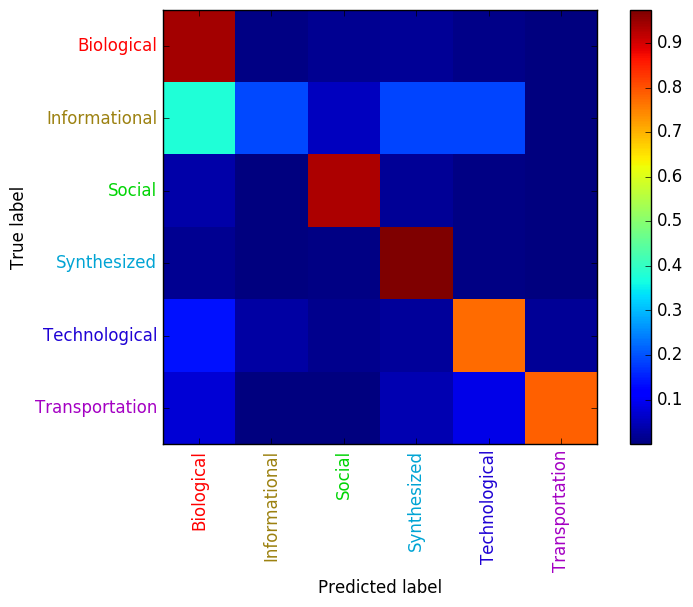
\includegraphics[width=\linewidth]{figs/similarity/Domain/None/confusion_None.png}
\caption{No sampling. Averaged accuracy: 90.68\%} \label{no_confusion}
\end{subfigure}\hspace*{\fill}
\begin{subfigure}{0.48\textwidth}
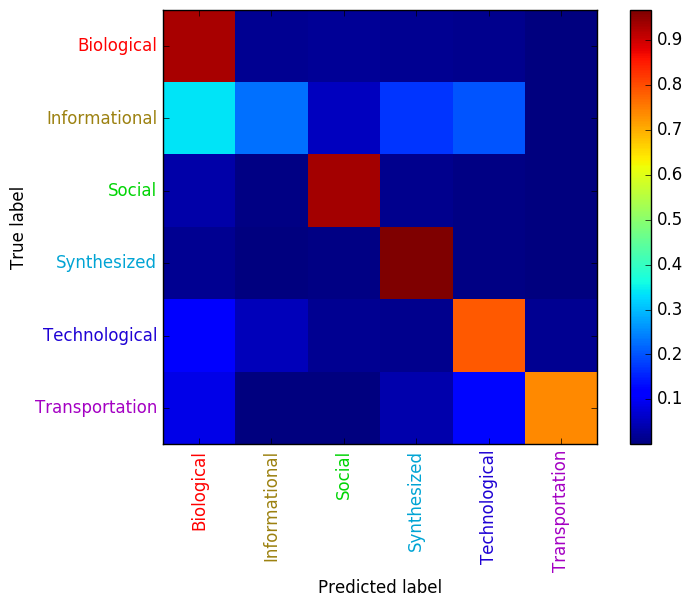
\includegraphics[width=\linewidth]{figs/similarity/Domain/RandomOver/confusion_RandomOver.png}
\caption{Random over-sampling. Averaged accuracy: 90.27\%} \label{random_over_confusion}
\end{subfigure}

\medskip
\begin{subfigure}{0.48\textwidth}
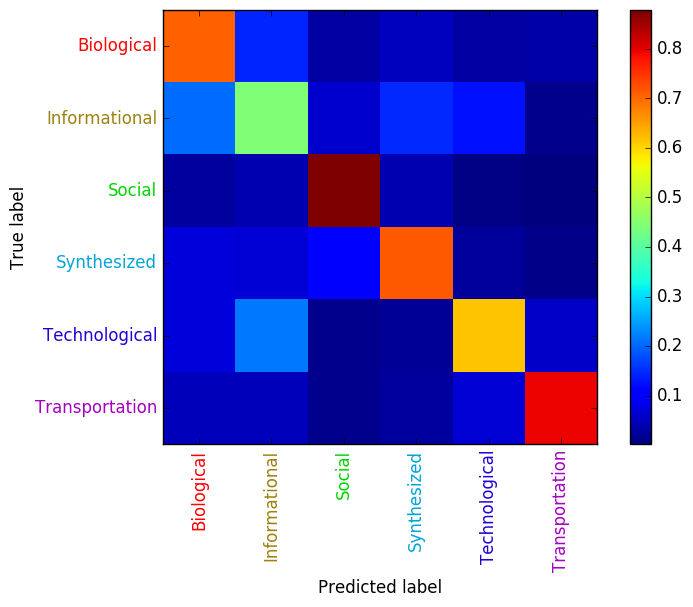
\includegraphics[width=\linewidth]{figs/similarity/Domain/RandomUnder_26/confusion_RandomUnder.png}
\caption{Random under-sampling. Averaged accuracy: 72.35\%} \label{random_under_confusion}
\end{subfigure}\hspace*{\fill}
\begin{subfigure}{0.48\textwidth}
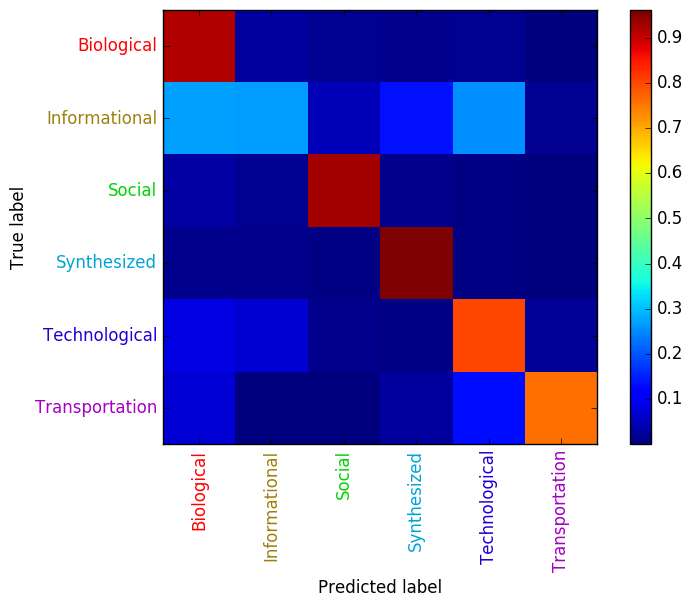
\includegraphics[width=\linewidth]{figs/similarity/Domain/SMOTE/confusion_SMOTE.png}
\caption{SMOTE. Averaged accuracy: 89.84\%} \label{smote_confusion}
\end{subfigure}
\
\caption{Confusion matrices for each of the sampling strategy. The color of each cell represents a count value normalized by the sum of all counts in a row the cell belongs to. Our similarity measurement is based on this normalized value of a confusion matrix.} \label{confusion}
\end{figure}

\begin{figure}[H]
\begin{subfigure}{0.48\textwidth}
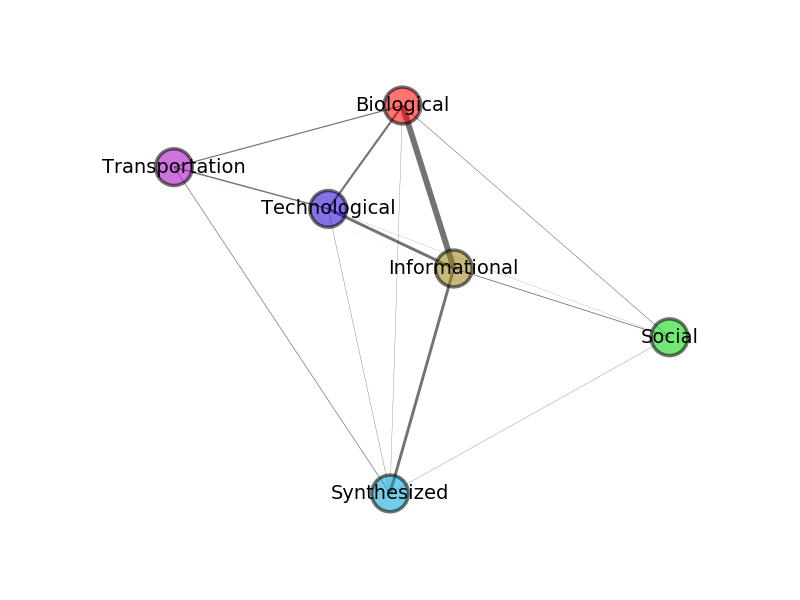
\includegraphics[width=\linewidth]{figs/similarity/Domain/None/g.png}
\caption{No sampling} \label{no_graph}
\end{subfigure}\hspace*{\fill}
\begin{subfigure}{0.48\textwidth}
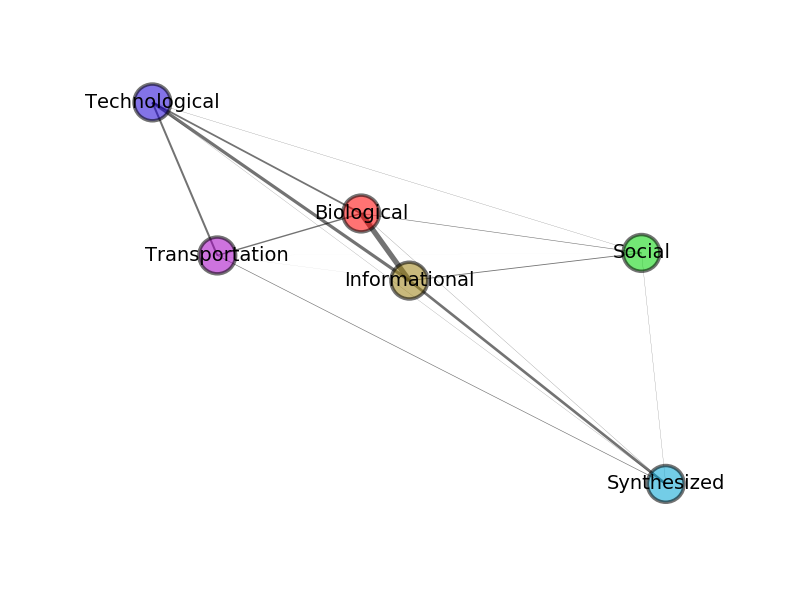
\includegraphics[width=\linewidth]{figs/similarity/Domain/RandomOver/g.png}
\caption{Random over-sampling.} \label{random_over_graph}
\end{subfigure}

\medskip
\begin{subfigure}{0.48\textwidth}
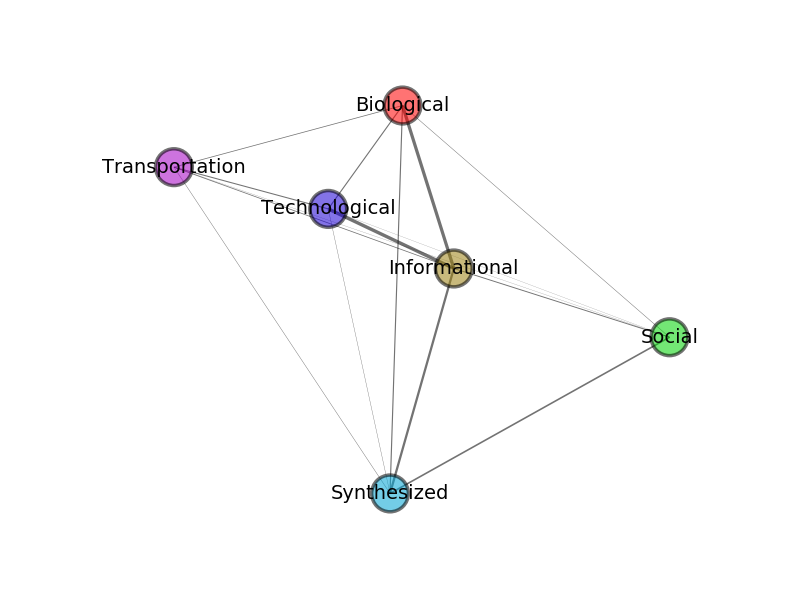
\includegraphics[width=\linewidth]{figs/similarity/Domain/RandomUnder_26/g.png}
\caption{Random under-sampling.} \label{random_under_graph}
\end{subfigure}\hspace*{\fill}
\begin{subfigure}{0.48\textwidth}
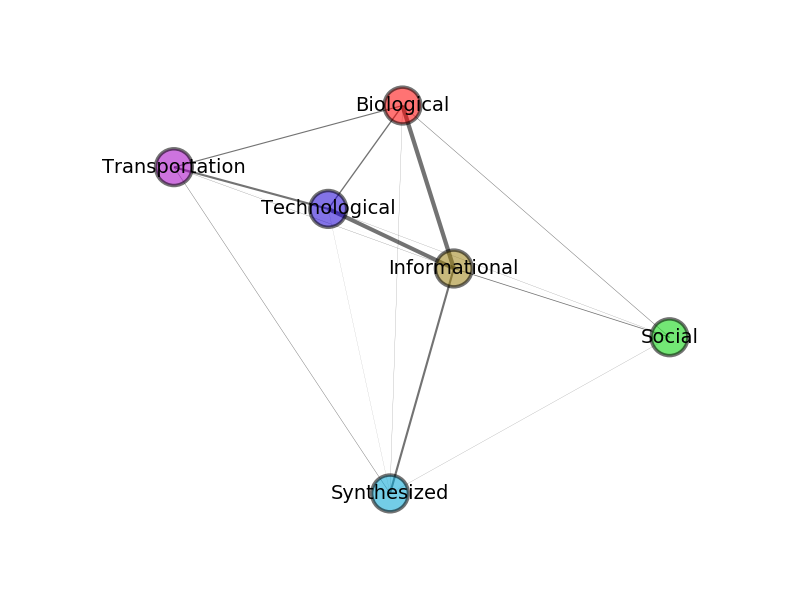
\includegraphics[width=\linewidth]{figs/similarity/Domain/SMOTE/g.png}
\caption{SMOTE.} \label{smote_graph}
\end{subfigure}
\
\caption{Meta networks for different sampling strategies. The widths of edges are proportional to the magnitude of the value in a symmetrized, normalized confusion matrix. Biological, Informational and Technological domains are well connected in all cases.} \label{meta_network}
\end{figure}


\subsubsection{Network Sub-domains}
Here we continue the same analysis as we have done in the previous section, but using network sub-domains as class labels for classification task.
Although in total we have 33 network sub-domains as shown in Fig. \ref{sub_dist}, some sub-domains have only few instances, which makes it infeasible to do classification task as it involves train-test split of data and SMOTE assumes a training set to have enough amount of instances for selecting $k$ nearest neighbors. Therefore we first exclude sub-domains that the number of instances within themselves are less than seven. This filtering results in 22 network sub-domains for this analysis. 

Same as the previous setting for network domain, we run classification tasks 1000 times for each sampling method, aggregate resulting confusion matrices, normalize and symmetrize them. Figure \ref{confusion_sub} shows the aggregated confusion matrices for each sampling method in which we can observe that all of the confusion matrices exhibit the diagonal pattern, an indication of underlying separability of network sub-domains. Note that, however, some sub-domains such as Bayesian, Web Graph, Offline Social, Water Distribution and Software Dependency, are often not classified correctly which may be due to the few instances and/or the fact that underlying structures of their instances are actually quite similar to ones of other sub-domains.

In order to visualize the underlying similarities within network sub-domain, we again construct meta networks of sub-domains based on a weighted adjacency matrix derived from aggregated confusion matrices, shown in Fig.\ref{meta_network}. From this figure, we can observe the network domain is not necessarily a good indicator of sub-domain clustering: informational networks including web graph, bayesian and peer to peer network and biological networks, such as metabolic, fungal, food web, etc. are not clustered together, meaning that we do not observe the sub-domains having the same color forming a community together. Then the question is: \textit{What could be a good indicator of similarity in networks of different kinds?} In order to answer this question, we first need to discover the communities of meta networks which are groups of nodes within which the edge density is high, but between which the edge density is low.

\begin{figure}[H]
	\begin{subfigure}{0.48\textwidth}
	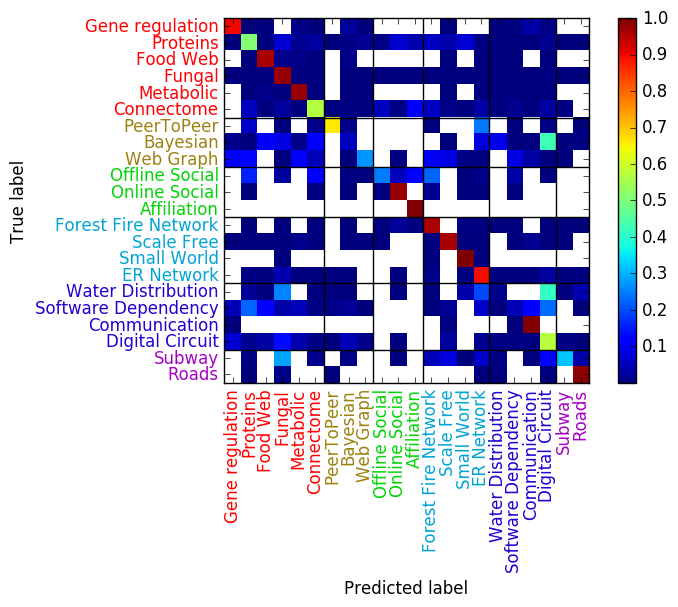
\includegraphics[width=\linewidth]{figs/similarity/SubDomain/None/confusion_sub_None.png}
	\caption{No sampling. Averaged accuracy: 89.45\%} \label{no_confusion_sub}
	\end{subfigure}\hspace*{\fill}
	\begin{subfigure}{0.48\textwidth}
	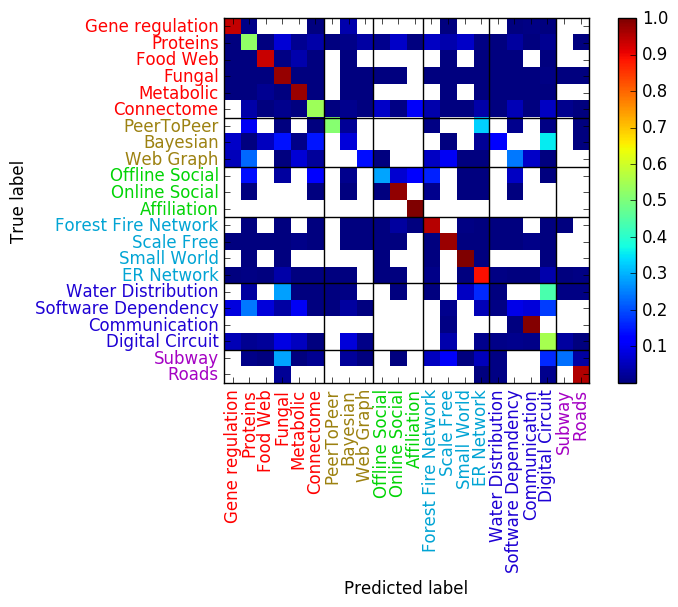
\includegraphics[width=\linewidth]{figs/similarity/SubDomain/RandomOver/confusion_sub_RandomOver.png}
	\caption{Random over-sampling. Averaged accuracy: 89.1\%} \label{random_over_confusion_sub}
	\end{subfigure}
	
	\medskip
	\begin{subfigure}{0.48\textwidth}
	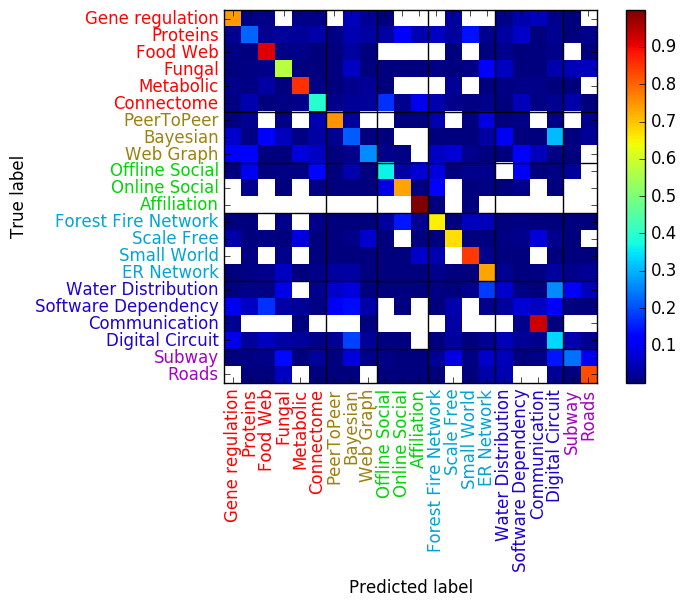
\includegraphics[width=\linewidth]{figs/similarity/SubDomain/RandomUnder_all5/confusion_sub_RandomUnder.png}
	\caption{Random under-sampling. Averaged accuracy: 69.23\%} \label{random_under_confusion_sub}
	\end{subfigure}\hspace*{\fill}
	\begin{subfigure}{0.48\textwidth}
	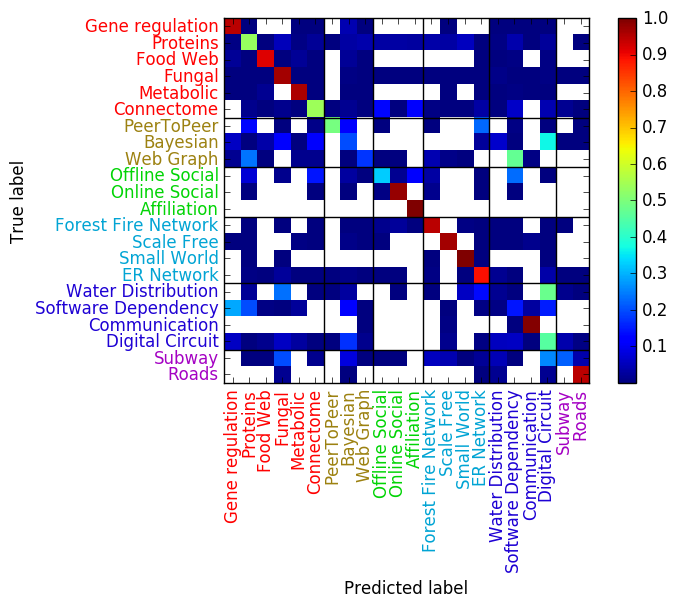
\includegraphics[width=\linewidth]{figs/similarity/SubDomain/SMOTE/confusion_sub_SMOTE.png}
	\caption{SMOTE. Averaged accuracy: 88.52\%} \label{smote_confusion_sub}
	\end{subfigure}
\
\caption{Confusion matrices for each of the sampling strategy. The white cells in confusion matrices indicate zero occurrence of corresponding classifications: sub-domain $i$ is misclassified as sub-domain $j$. The color of each cell represents a count value normalized by the sum of all counts in a row the cell belongs to. Our similarity measurement is based on the normalized value of a confusion matrix shown in above. Lines within confusion matrices indicate the separations of network domains.} \label{confusion_sub}
\end{figure}

\begin{figure}[H]
	\begin{subfigure}{0.48\textwidth}
	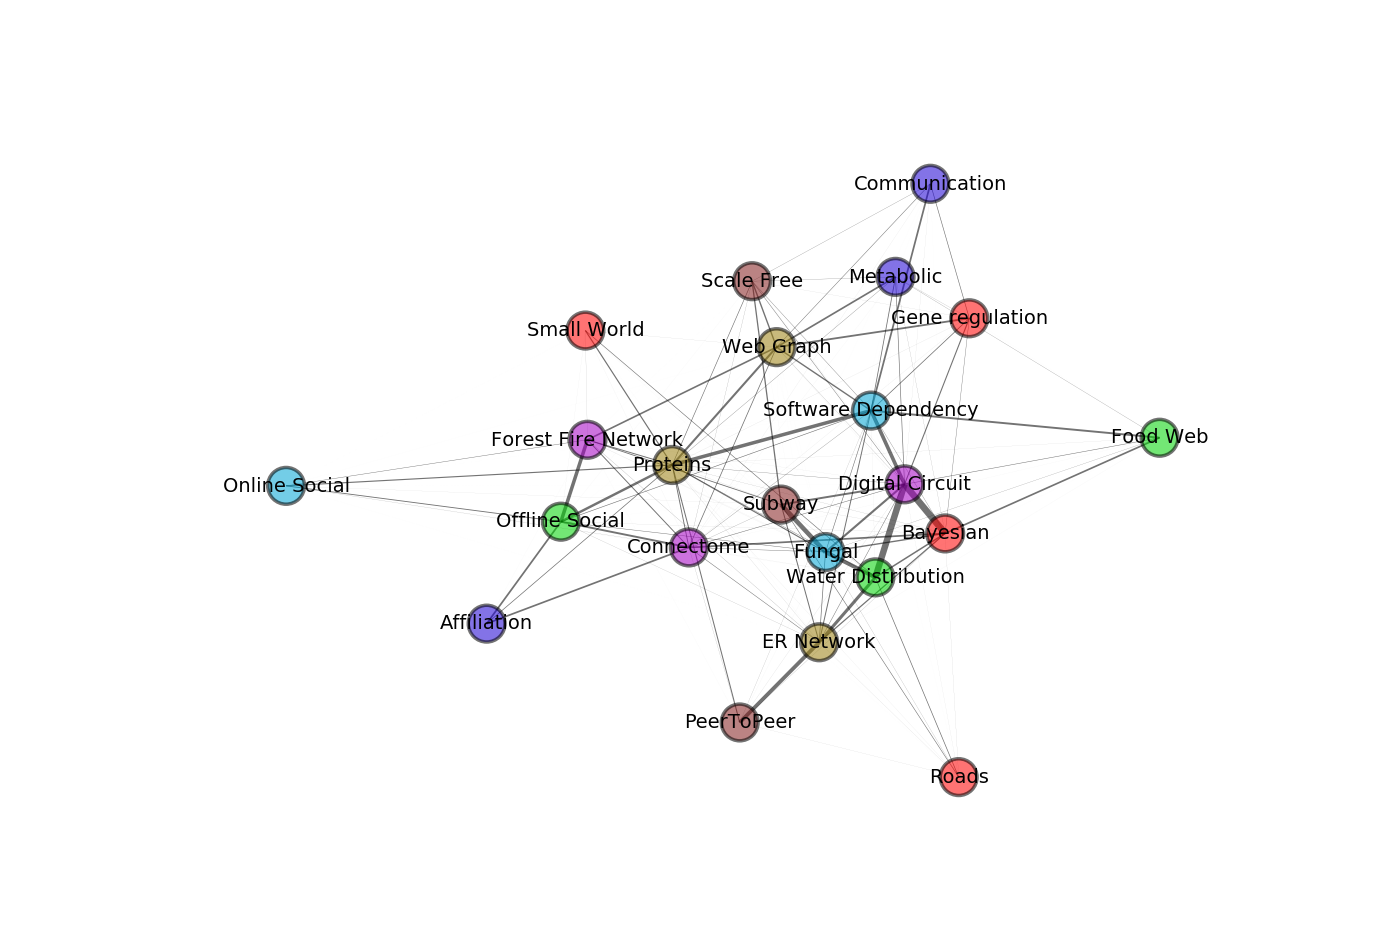
\includegraphics[width=\linewidth]{figs/similarity/SubDomain/None/g.png}
	\caption{Meta network based on no sampling.} \label{no_graph_sub_original}
	\end{subfigure}\hspace*{\fill}
	\begin{subfigure}{0.48\textwidth}
	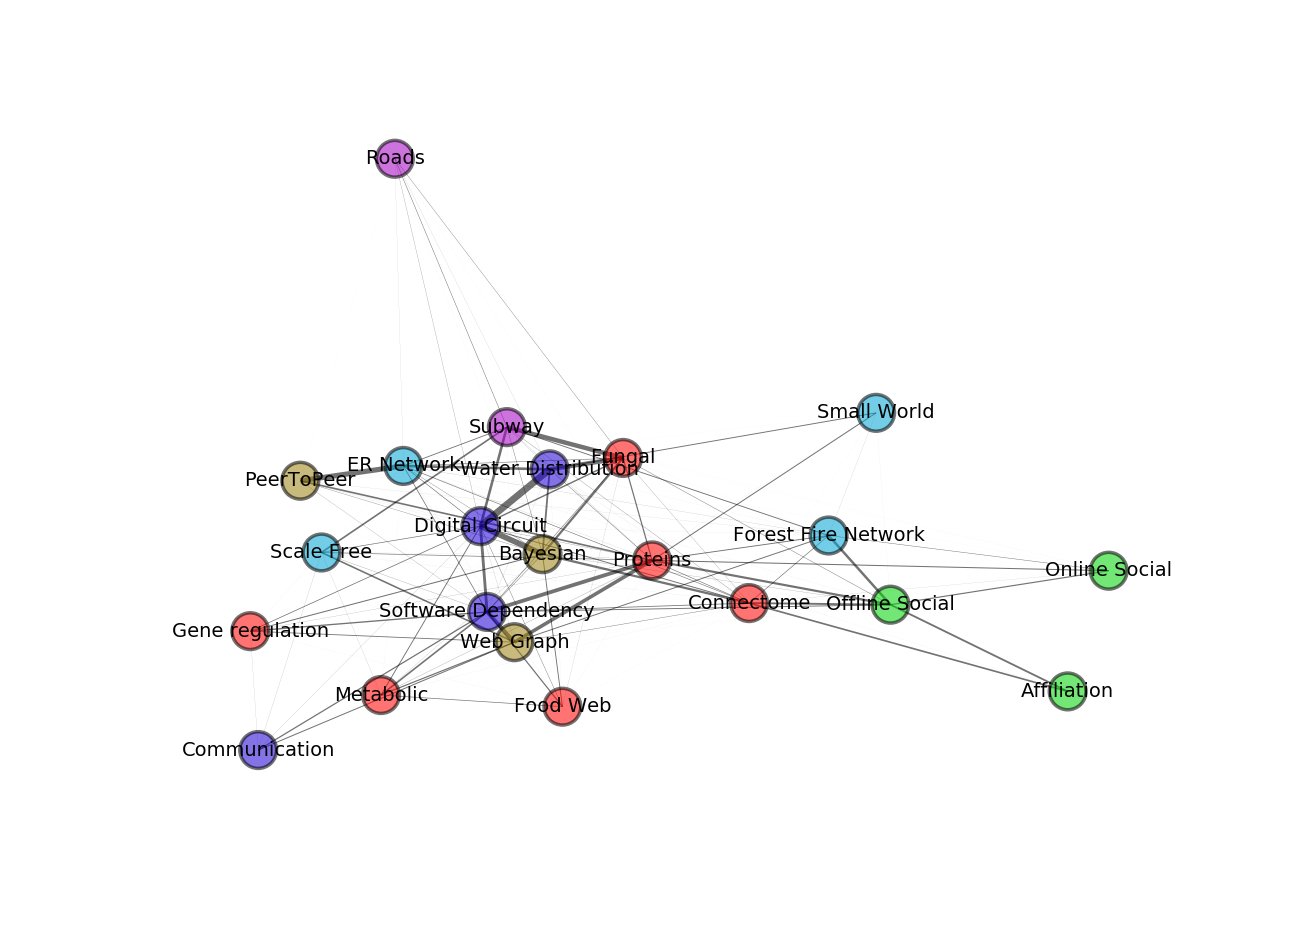
\includegraphics[width=\linewidth]{figs/similarity/SubDomain/RandomOver/g.png}
	\caption{Meta network based on random over-sampling.} \label{random_over_graph_sub_original}
	\end{subfigure}
	
	\medskip
	\begin{subfigure}{0.48\textwidth}
	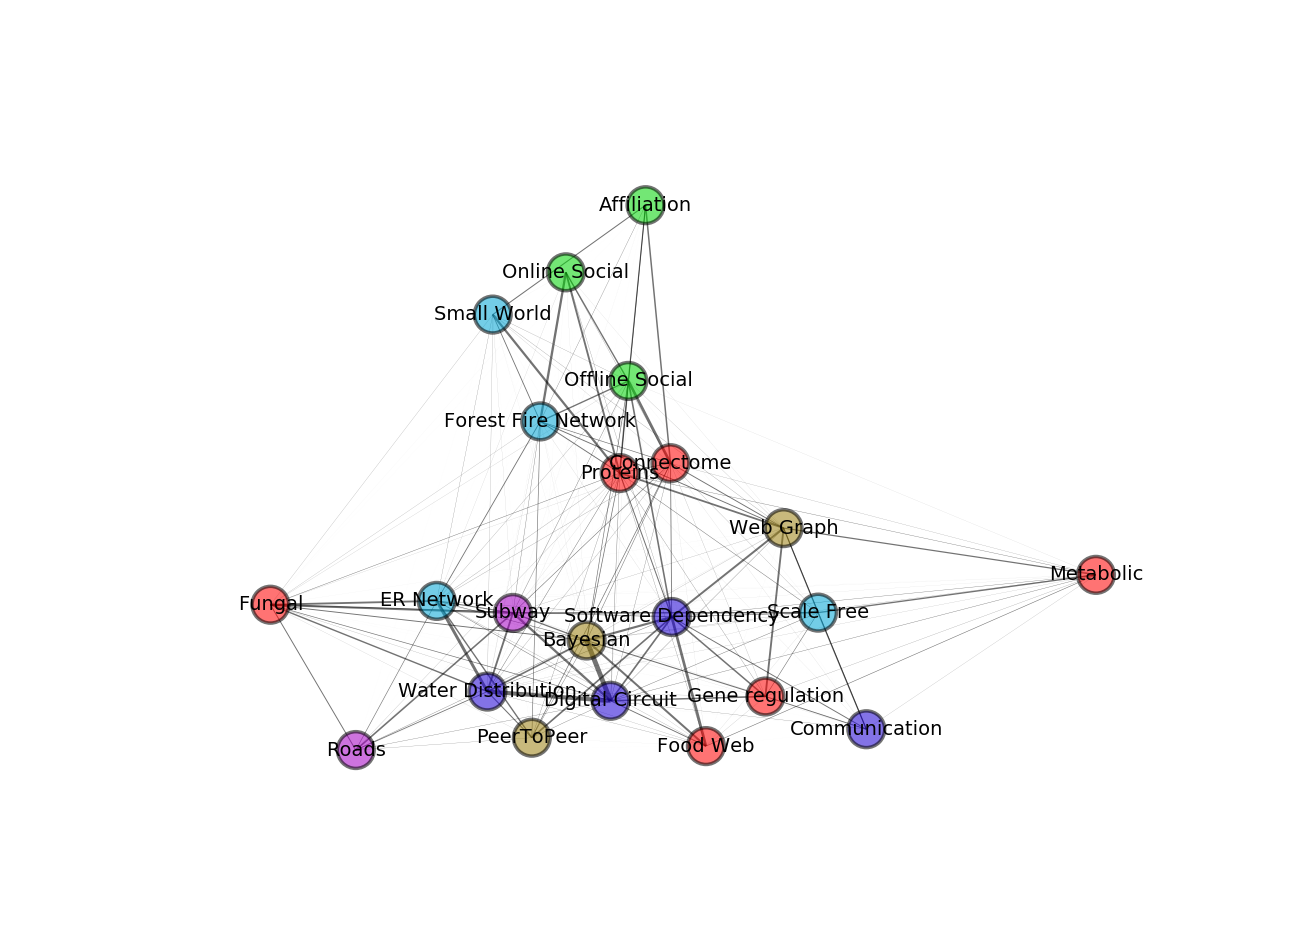
\includegraphics[width=\linewidth]{figs/similarity/SubDomain/RandomUnder_all5/g.png}
	\caption{Meta network based on random under-sampling.} \label{random_under_graph_sub_original}
	\end{subfigure}\hspace*{\fill}
	\begin{subfigure}{0.48\textwidth}
	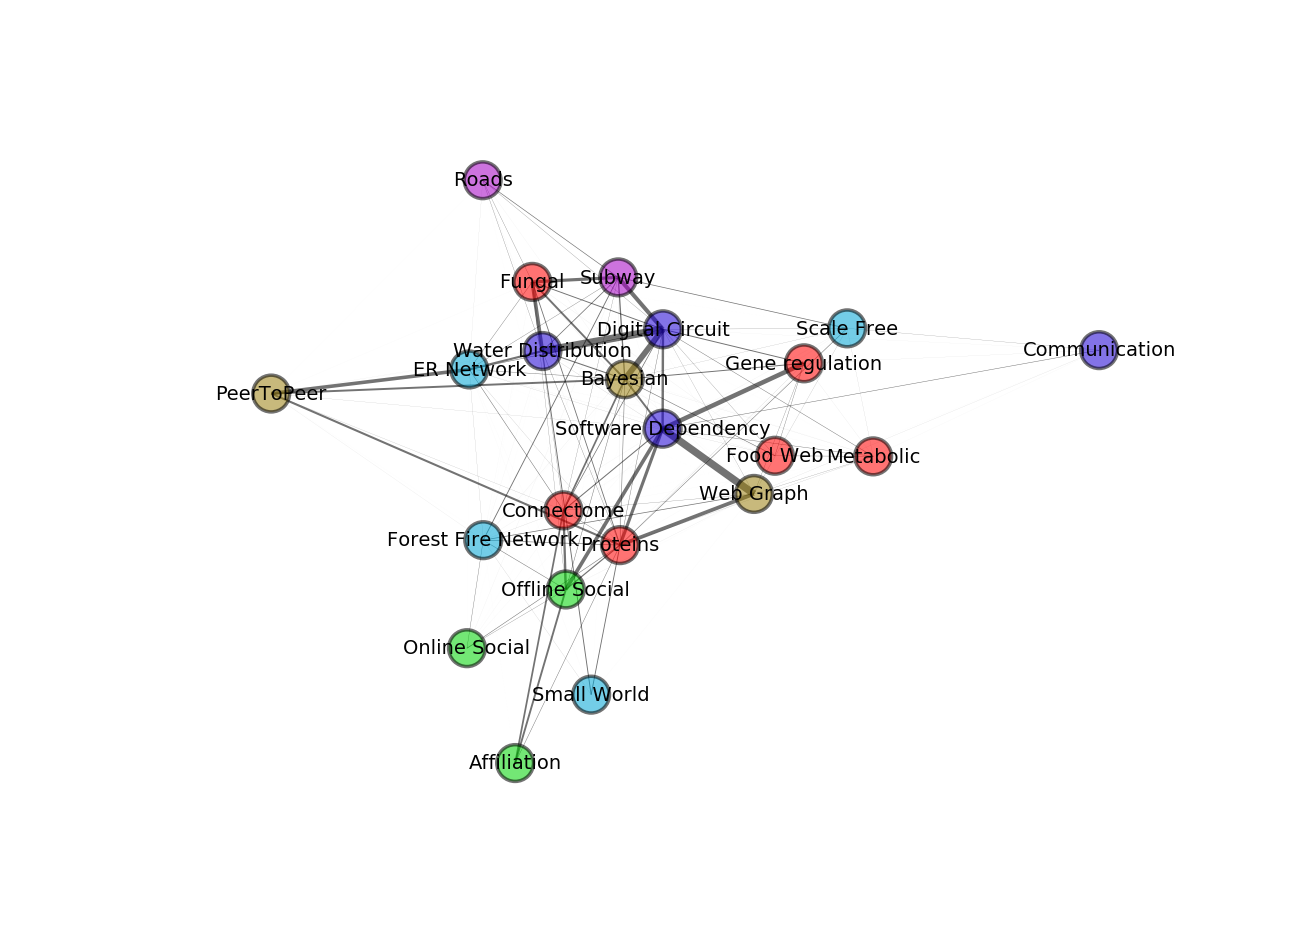
\includegraphics[width=\linewidth]{figs/similarity/SubDomain/SMOTE/g.png}
	\caption{Meta network based on SMOTE.} \label{smote_graph_sub_original}
	\end{subfigure}
\
\caption{The meta networks of network sub-domains. The color of each node corresponds to a domain the sub-domain (node) belongs to.} \label{meta_network}
\end{figure}

\begin{figure}[H]
	\begin{subfigure}{0.48\textwidth}
	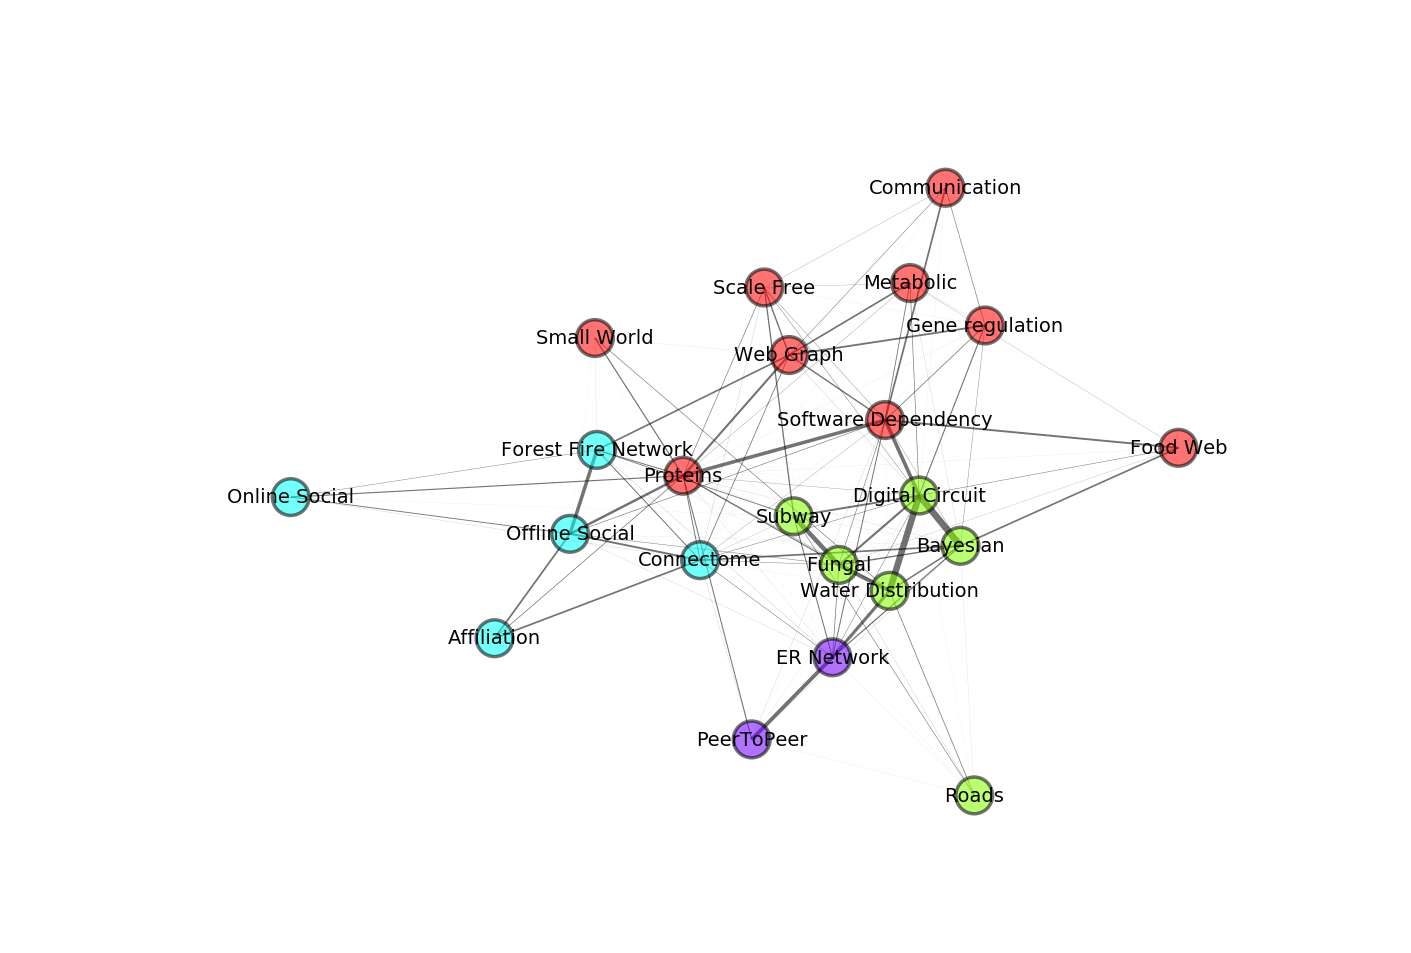
\includegraphics[width=\linewidth]{figs/similarity/SubDomain/None/g_community.png}
	\caption{Meta network based on no sampling. The number of communities is $4$.} \label{no_graph_sub_community}
	\end{subfigure}\hspace*{\fill}
	\begin{subfigure}{0.48\textwidth}
	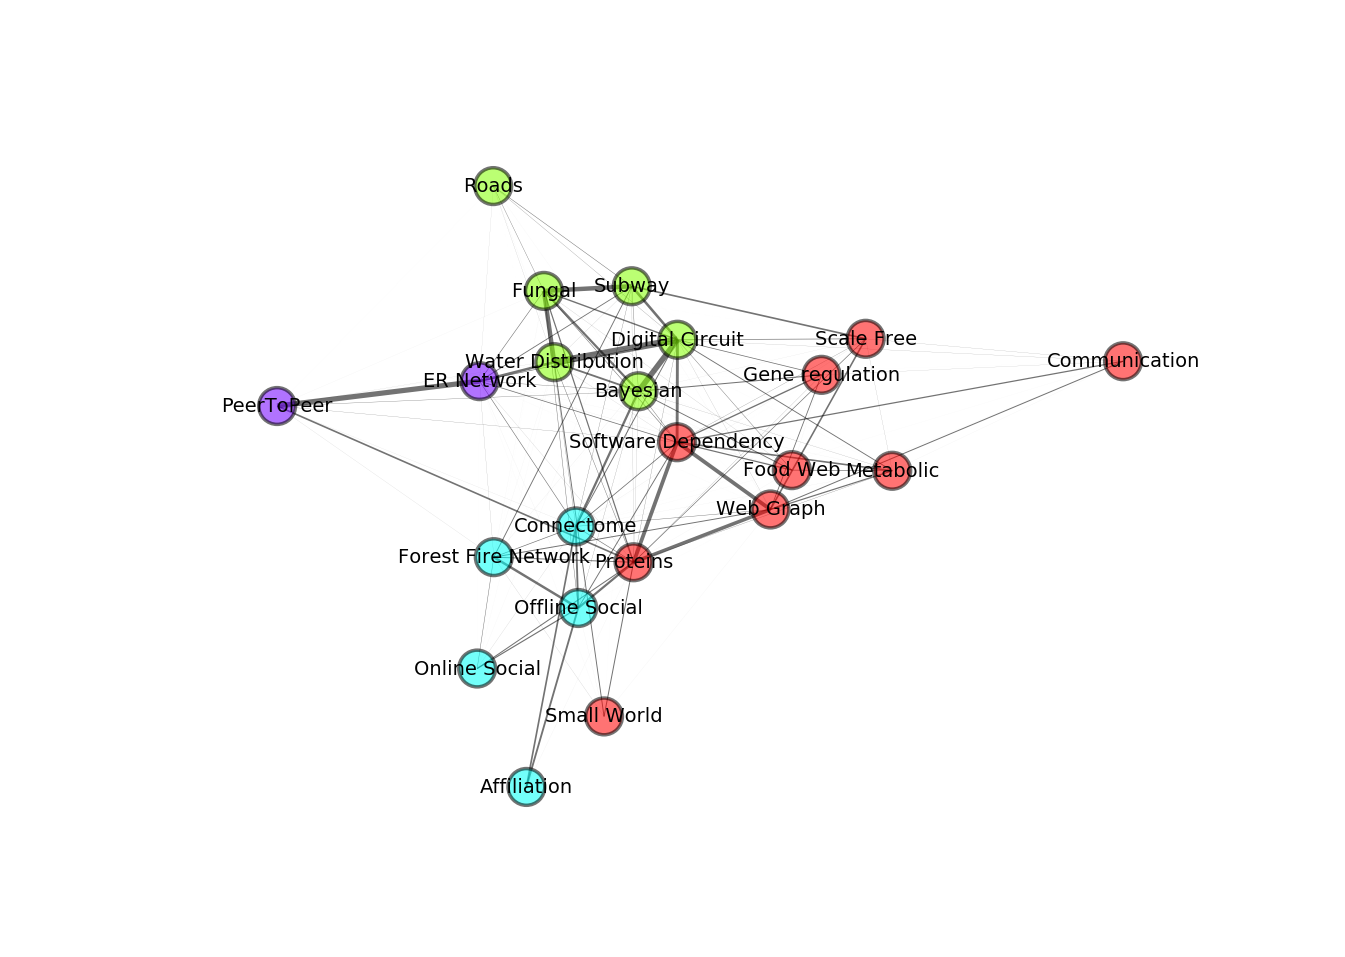
\includegraphics[width=\linewidth]{figs/similarity/SubDomain/RandomOver/g_community.png}
	\caption{Meta network based on random over-sampling sampling.  The number of communities is $4$.} \label{random_over_graph_sub_community}
	\end{subfigure}
	
	\medskip
	\begin{subfigure}{0.48\textwidth}
	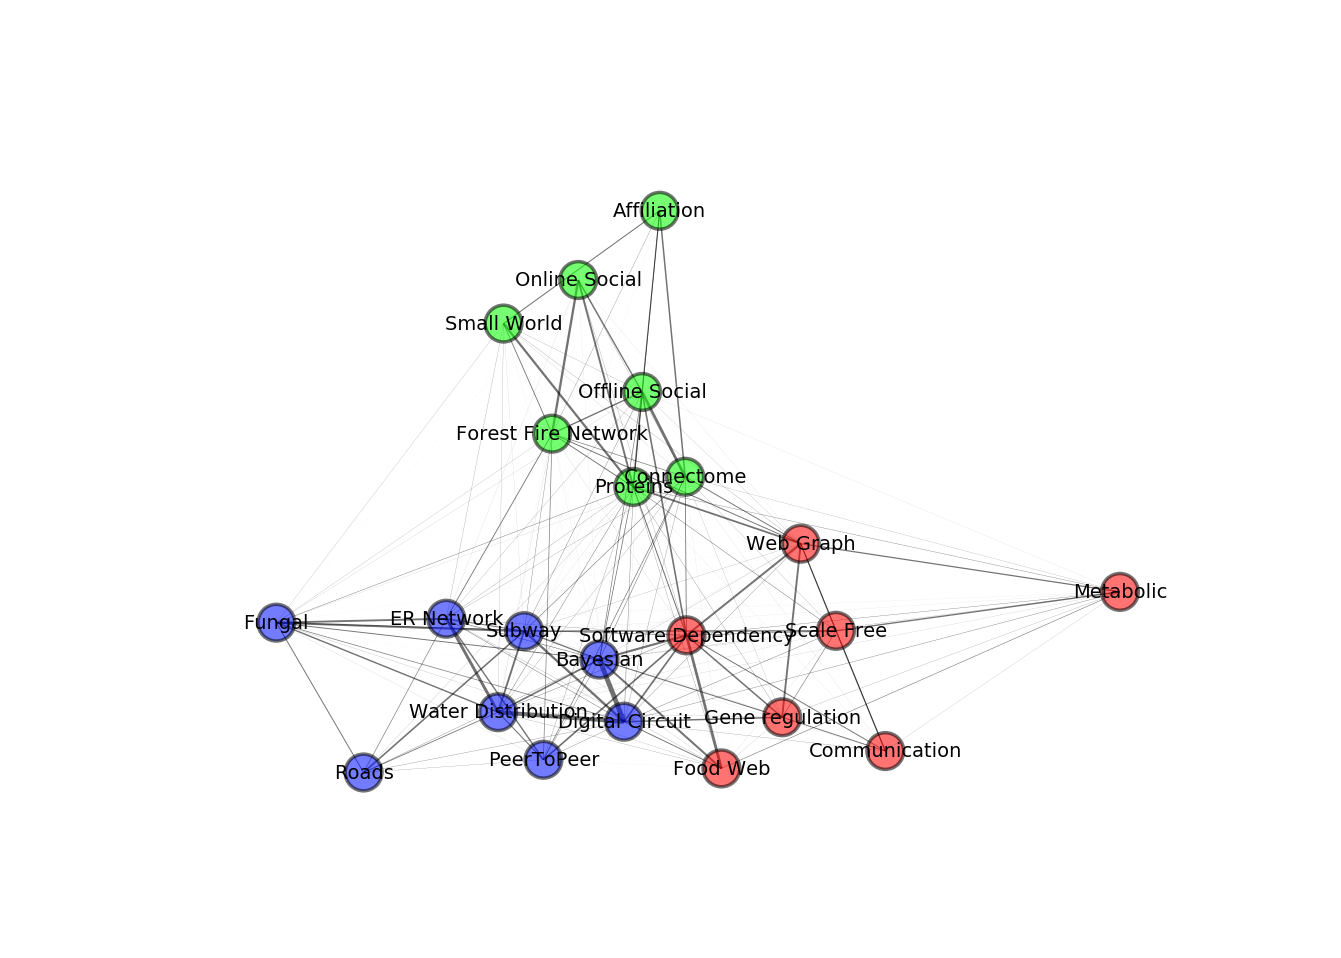
\includegraphics[width=\linewidth]{figs/similarity/SubDomain/RandomUnder_all5/g_community.png}
	\caption{Meta network based on random under-sampling.  The number of communities is $3$.} \label{random_under_graph_sub_community}
	\end{subfigure}\hspace*{\fill}
	\begin{subfigure}{0.48\textwidth}
	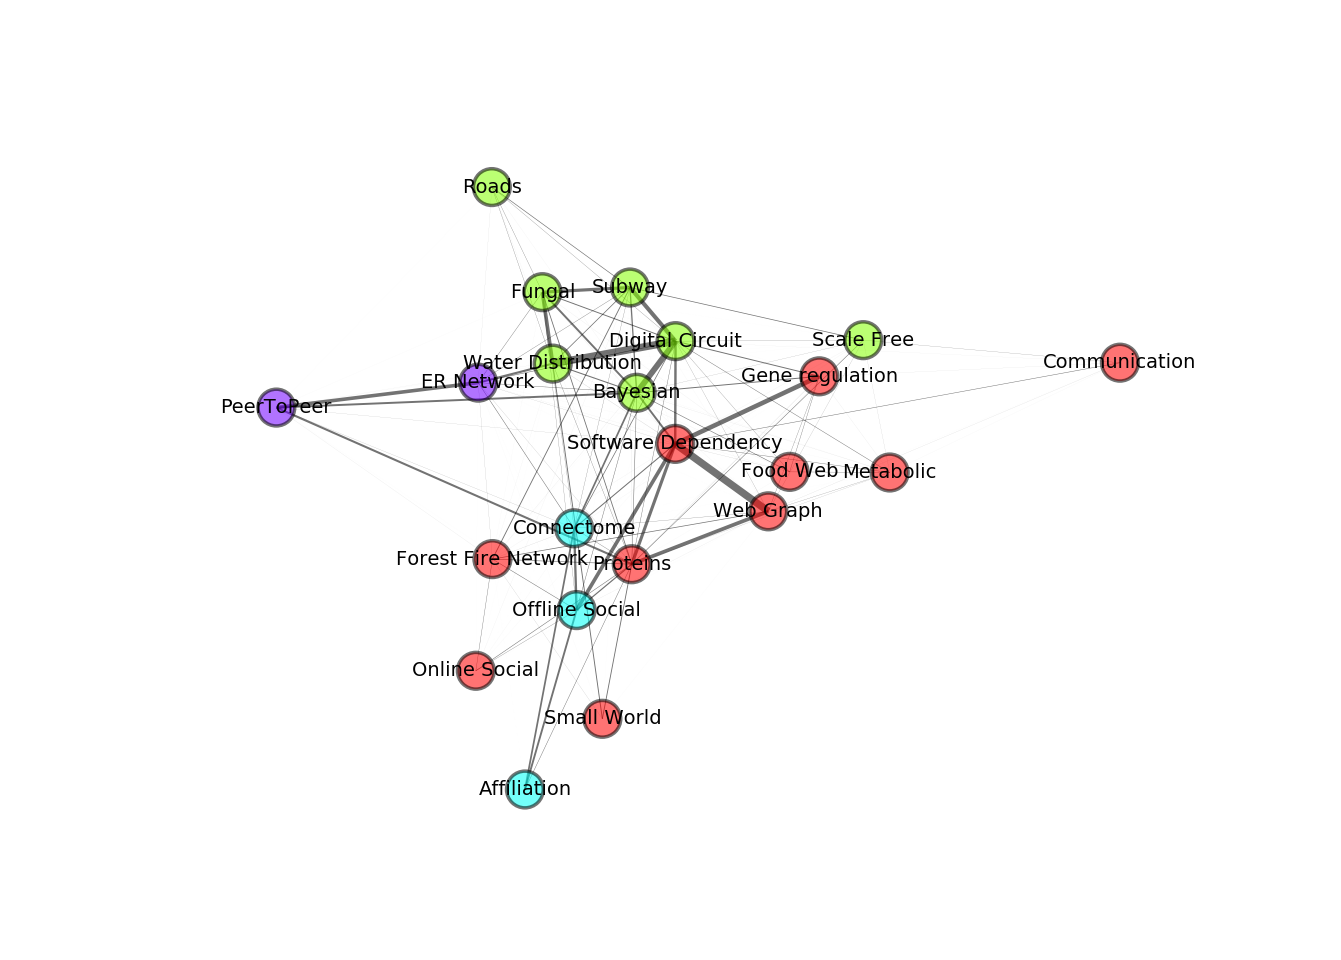
\includegraphics[width=\linewidth]{figs/similarity/SubDomain/SMOTE/g_community.png}
	\caption{Meta network based on SMOTE.  The number of communities is $4$.} \label{SMOTE_graph_sub_community}
	\end{subfigure}
\
\caption{The meta networks of network sub-domains with community labelings. The color of node now corresponds to a community found by the algorithm.} \label{meta_network_community}
\end{figure}

Fig.\ref{meta_network_community} shows the meta networks of sub-domains on which the colors of nodes correspond to the community membership that is found by a community detection algorithm proposed by Clauset \textit{et al.} \cite{CNMAlgorithm}. We have used the implementation of the modified version of this algorithm for weighted network that is available in Python-igraph as a method \texttt{community\_fastgreedy()} \cite{igraph}. From the figure \ref{meta_network_community}, one may notice that the community structure across different sampling methods is almost consistent, meaning the certain groups of sub-domains are always in the same community.  For instance, for all sampling methods, offline social, connectomel and affilication networks are in the same community. Some network sub-domains, however, change the community membership for some meta networks. For instance, online social network and forest fire model networks join the community of off-line social network for no sampling, random-over sampling and random-under sampling method, but joins the community of software dependency (red color) for SMOTE sampling. This variation of community membership across all meta networks can be expressed in a diagram shown in the figure \ref{community_overlaps}. In this figure sub-domains that are in the same community at least for one meta network are in the same circle. From this diagram, one can notice the underlying principles of the community structure: these communities correspond to the functionality, constraints and growing mechanism of networks. The sub-domains of the left side especially the ones consistently clustered together, such as digital circuit bayesian networks, water distribution networks, etc., seem to have a common property among them: they are some sort of a "flow" network. A list of such flow includes: electrical signal (digital circuit), information (bayesian), water (water distribution), nutrient (fungal), people/trains (subway) and cars (road). Also, if we look at the meta networks, digital circuit and bayesian networks are always tightly connected together. This may be due to the fact that they are both an input-output network as well as being a flow network. The rest of the flow networks have another common property, that is, physical embedding of the network. These networks have a strong constraint of the physical limitation. For instance, it is almost impossible for a node in a physically embedded network to have a thousand connections upon it.

The sub-domains of the right circle, again the ones consistently clustered together including software dependency, protein interactions, web graphs, scale-free and communication, except small world network, appear to have the same growing mechanism of the network, namely preferential attachment. If a network grows according to preferential attachment, newly added nodes, for example newly created web page or software package, tend to connect to the popular or high-degree nodes, i.e. popular web sites or widely used software packages. 

The circle at the top contains online social, offline social and forest fire model networks. The fact that these three sub-domains are always clustered together without having any other sub-domain in the same community implies that the strong characteristic of social networks as pointed out in a number of studies and the validity of forest fire model for modeling such social networks.

\begin{figure}[ht]
		\begin{center}
		\vspace{0.5cm}
		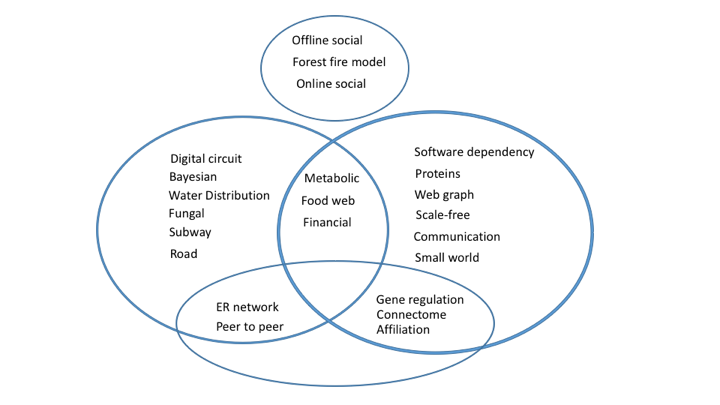
\includegraphics[clip,width=12cm,height = 6cm]{figs/community_overlaps.png}
		\vspace{0.5cm}
		\caption{Overlaps of community memberships. Each circle in this figure means that sub-domains in the circle are in the same community for a meta network corresponding to a specific sampling method. Online social, offline social and forest fire networks are in the same community across all meta networks. Sub-domains on the left circle including digital circuits, bayesian networks, etc., are consistently in the same community with some other sub-domains, such as ER network and metabolic network, joining the community. The same phenomenon is observed for the community of software dependency, proteins, etc., that corresponds to the circle on the right side.}
		\label{community_overlaps}
 		\end{center}
\end{figure}

The intersections of community overlap circles are where some ambiguity remains. Metabolic network, for example is at the intersection of flow networks and preferential attachment networks. It is known that metabolic network is in fact a so-called scale-free network and the preferential attachment mechanism can be explained by the natural selection over the course of evolution. However, one can think metabolic network as some sort of flow network having some input-output relations as well: the input corresponds to nutrients and they get broken down into pieces of chemical; the output corresponds to the usable chemical compound that a living organism needs in order to survive. Therefore, it is reasonable for this factory-like flow network to be classified as or similar with other flow networks such as digital circuit or bayesian networks as well as a preferential attachment network. 

Our findings from this experiment provide some supporting evidence that the network structure is indeed is influenced by the underlying function, constrain and growing mechanism of the network. 


%%%%%%%%%%%%%%%% --- New Chapter --- %%%%%%%%%%%%%%%%
\newpage
\section{Discussion}
In the previous chapter, we have found the distinguishing features for various network sub-domains with possible explanations for the underlying processes of networks, and the hidden similarities among network domains and sub-domains based on meta networks we have constructed. In this chapter we are going to synthesize the our findings and the previous studies together.

In the investigation of distinguishing features and the separability of sub-domains, we have observed that some network sub-domains are hard to be separated in the feature space, which can be also seen in AUC score. This finding has an interesting connection with the meta networks we have constructed later: the sub-domains having high separability, such as online social networks and ecological food-webs, tend to be at the \textit{periphery} of the meta networks, whereas the subdomains having low separability, such as protein interaction networks and metabolic networks, tend to be at the \textit{core} of the meta networks. In the meta networks, the core of nodes essentially depicts the sub-domains that are frequently misclassified by a classifier due to their structural similarity and the periphery displays sub-domains that are dissimilar to other sub-domains in terms of network structure. Therefore, it is relatively easy to infer that the sub-domains at the core that were not studied for finding the distinguishing features, such as digital circuits and web graphs, may also exhibit low separability in the feature space. 


 As we have seen in confusion matrices in the figure \ref{confusion}, network domains such as Biological, Social, etc. are quite separable in the feature space. Also, confusion matrices of network sub-domains exhibit the strong diagonal patterns except few such as bayesian network and web graphs, indicating the separability of networks at the sub-domain level. These separabilities of networks in the different levels (domain and sub-domain) tells us something about the \textit{manifold} of networks in the high dimensional feature space: in the feature space at the domain level, points that corresponds to individual networks in the same network domain make a manifold of an intricate shape. Each sub-domain in the specific domain forms a part of the entire manifold and the volume it covers may overlap with the one covered by the other. The confusion matrices for classification of network domain essentially indicates that manifolds, each corresponds to a network domain, reside in some region of the feature space with some overlaps with each other. If we decompose the manifolds into manifolds of network sub-domains, we see a different outcome. Some sub-domains in a network domain occupy some regions of the feature space that are completely separated; they correspond to the non-overlapping section of manifolds at the level of network domain. They include, for example, food webs for Biological, peer to peer for Informational, communication for Technological and roads for Transportation. Some network sub-domains, however, almost completely overlap in the feature space with other sub-domains, and they correspond to the overlapping section of manifolds at the network domain level. They include bayesian and web graphs for Informational and water distribution and software dependency for Technological. 


This idea of thinking networks in a feature space as a manifold of complex shape has some previous studies. Avena-Koenigsberger \textit{et al.} have studied the idea of \textit{network morphospace} in which each axis corresponds to some feature related to the structure of networks, such as tree-ness, feed-forward ness and orderability \cite{NetworkMorphospace}. In this study, it is shown that different kinds of networks, such as technological, language and neural networks occupy some regions in the morphospace. One may notice in this study that some regions in morphospaces are not occupied at all by any networks. This observation gives us some question about the feature space: \textit{Are some regions of a feature space not habitable at all?} This question may be answered with the study done by Ugander \textit{et al.} \cite{Ugander:2013}. They have studied a feature space in which each axis corresponds to the sub graph frequency of networks and mathematically proved that there are some regions in the feature space that are not habitable at all. Interestingly, they observed that the real world networks, in this case Facebook networks, only occupy some parts of the habitable space. Taken together, these studies suggest that networks in the high dimensional feature occupy some regions of the entire possible space that is theoretically feasible. This phenomenon may be due to the fact that the space not occupied yet theoretically feasible corresponds to an inefficient structure of a network. Many of the biological networks and technological networks are optimized for a functioning by either natural selection over the course of evolution or effort of designing by a number of engineers and this may push the networks into a certain region in the feature space that happens to be occupied by the both kinds of networks. This is supported by one of our findings that fungal network, a kind of biological network developed by the evolutionary strategy, and water distribution networks, a kind of network designed by engineers, are structurally similar and their optimization is essentially for efficient flow on the network and cost-reduction of wiring.
 
 
 %%%%%%%%%%%%%%%% --- New Chapter --- %%%%%%%%%%%%%%%%
\newpage

 \section{Conclusion}
 In this thesis we have studied over 1000 real-world networks along with over 500 synthesized networks in order to understand the structure of complex networks across various domains and sub-domains. Our study successfully identified the distinguishing features for network sub-domains including protein interaction, metabolic, ecological food web, connectome, online social and communication networks and found out some of these features can naturally explain the process in the network of interest. Using machine learning techniques such as random forest classifier, confusion matrix and community detection algorithm, our study uncovered the underlying principles of network structure: the functionality, constraint and growing mechanism of a network play an important role for construction of networks having certain structural properties.
 
 
 %%%%%%%%%%%%%%%% --- New Chapter --- %%%%%%%%%%%%%%%%
\newpage

\section{Future Work}
There is still some room for our study to be improved. The class imbalance problem, even though we have utilized sampling methods in order to alleviate the problem, is the main remaining concern. Since we have discarded some network sub-domains due to the lack of instances needed for classification tasks, we could possibly discover other hidden properties and relationships if more instances for such sub-domains including language network, collaboration network, power grid network and so on. Another direction for future research is incorporating other scale-invariant structural features. In this study we have only used a set of eight features. It is possible, however, that adding other dimensions in the feature space may reveal other hidden properties that were not captured in our feature set.

\clearpage

\bibliographystyle{ieeetr}
\bibliography{reference} 

\end{document}












 
 